\documentclass[a4paper]{book}

\usepackage[utf8]{inputenc}
\usepackage[english,russian]{babel}
\selectlanguage{russian}
\usepackage{listings}
\usepackage{hyperref}
\usepackage{underscore} % no need to escape underscore with this pack
\usepackage[dvips]{graphicx}
\usepackage{babel}
\usepackage{verbatim}   % multi-line comments
%\usepackage{sectsty}
%\usepackage[normalem]{ulem}
%\usepackage{indentfirst}
%\usepackage{amsfonts}
%\usepackage{fancyhdr}
%\pagestyle{fancy}

\renewcommand{\labelenumii}{\asbuk{enumii})}

\def\tn{т.\thinspace н.}
\def\td{т.\thinspace д.}
\def\tp{т.\thinspace п.}
\def\to{т.\thinspace о.}
\def\To{Т.\thinspace о.}
\def\te{т.\thinspace е.}
\def\Te{Т.\thinspace е.}
\def\itd{и т.\thinspace д.}
\def\ur{Uranium}
\def\na{named\_arg*}

\graphicspath{{pics/}}

\lstnewenvironment{example}[2]%
   {%
    \minipage[t]{0.9\linewidth}%
    \lstset{language=Prolog, frame=single, breaklines=true,%
            breakatwhitespace=true,%
            basicstyle=\small,%
            frameround=fttt,frame=trBL,%
            caption={#1},label={#2}}%
   }%
   {\endminipage\smallskip}

\lstnewenvironment{bigexample}[2]%
   {%
    \lstset{language=Prolog, frame=single, breaklines=true,%
            breakatwhitespace=true,%
            basicstyle=\small,%
            xrightmargin=0.05\linewidth,%
            xleftmargin=0.05\linewidth,%
            frameround=fttt,frame=trBL,%
            caption={#1},label={#2}}%
   }%
   {\smallskip}

\lstnewenvironment{genexample}[2]%
   {%
    \minipage[t]{0.9\linewidth}%
    \lstset{frame=single, breaklines=true,%
            breakatwhitespace=true,%
            basicstyle=\small,%
            frameround=fttt,frame=trBL,%
            caption={#1},label={#2}}%
   }%
   {\endminipage\smallskip}

\begin{document}
\title{{\bf\ur}\\ \medskip  Пролог-библиотека для автоматизации
  тестирования ПО}
\author{Сергей Лодягин\\ \texttt{lodyagin@gmail.com}}
\date{\today}
\maketitle

\tableofcontents

\part{Введение в автоматизацию с помощью \ur}

\chapter{Предисловие}

Разработка программного обеспечения всегда являлась отраслью, где
инновации часто рождались и умирали в рамках жизни одного
проекта. Но методики, которые сегодня можно назвать
классическими, проходили проверку временем и совершенствовались
десятилетиями. Они давали начала различным
технологиям. Технология позволяла применять отлаженную схему,
группу методик при разработке различных проектов одной группой
разработчиков. Некоторые методики стоят ещё выше технологий,
например, методики тестирования программы или анализа алгоритмов
и являются универсальными.

В последние 10 лет в программировании наметилась тенденция
оформления различных принципов разработки и оформление их как
готовых решений. Например, семейство методик X. Даже программные
продукты, сопровождающие разработку и призванные быть гибким
инструментом позиционируют себя как относящиеся к тому или иному
пакету. И когда вам надо средство тестирования X вам надо и
система учётов дефектов X, и коммуникация X и \td, вплоть до
готовых групп разработчиков X со специального вида X-досками и
X-картами.  Зачастую тоже относится и к языкам программирования,
выбор которых предопределён существующей модой если не
предписаниями гуру от всепоглощающей методики.

Данное положение, являющееся сейчас едва ли не доминирующем во
всей отрасли, создаёт благоприятную почву для возвращения к
проверенным старым технологиям, и, если удаётся такую технологию
пустить в плавание по новому руслу, то зачастую может оказаться,
что добротные суда легко обходят наскоро сколоченные новые
посудины (хотя бы потому, что могут ходить как по так и против
течения).

Одной из таких проверенных временем технологий является язык
Пролог, разработанный французом Аланом Колмерау (Alain Colmeraue)
в 1972~г.

Данная книга является, с одной стороны руководством по системе
тестирования \ur, которая написана на языке Пролог, а с другой
стороны демонстрацией того, как можно использовать проработанные
наукой теории (логику первого порядка, на принципах которой
построен сам язык Пролог) при решении реальных бизнес задач. В
качестве примера выбрана довольно распростанённая и насущного
среди (мелких) компаний задача тестирования интернет-магазина.

Вообще, следует сказать, что Пролог, ввиду своей исключительной
логической гибкости, очень хорошо подходит для последовательного
решения задач и не требует предварительного проектирования, а
потому является, пожалуй, королём прототипов; основной способ
проектирования программы в Прологе --- эволюционный, путём
постоянных запросов и дописания необходимых предикатов является
идеально настроенным на получение наискорейшей цели, что является
важным, когда нам надо протестировать работу программы.

\chapter{Учебный объект}

В качестве примера выбран магазин
\url{http://all-for-skin-beauty.com}, созданный советскими
иммигрантами. Магазин продаёт различные средства по уходу за
кожей и публикует статьи по той же тематике.

Структуру магазина можно изобразить следующей диаграммой.

\begin{figure}[h!]
\center{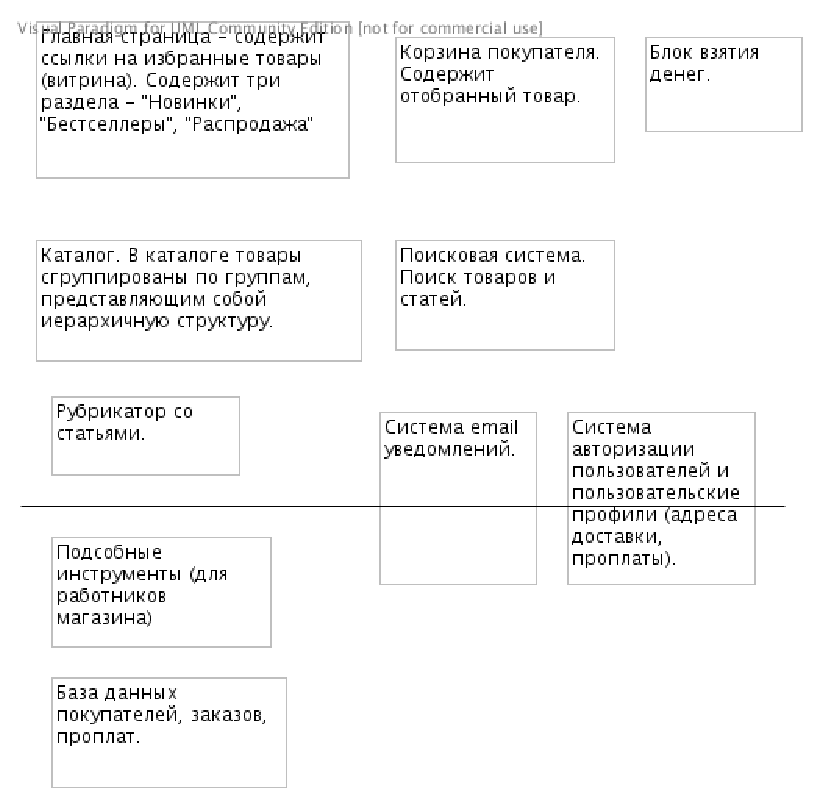
\includegraphics[width=1\linewidth]{eshop}}
%\caption{}
\label{eshop}
\end{figure}

Часть выше ватерлинии доступна покупателю, ниже - работникам
магазина. Поскольку магазин является роботом, он являет собой
любопытный экземпляр для тестирования - мы можем совершать
виртуальные заходы и наборы корзин и, если договоримся с
администрацией - даже виртуальные покупки виртуальными деньгами
(главное, не мешать основной массе покупателей, создавая высокую
нагрузку на сервер).


\chapter{Постановка задачи тестирования в современных условиях}

Нет более игнорируемой составляющей работ по тестированию равно
как и вообще, работ по обеспечению качества, чем определение
критериев качества, которые желает получить заказчик. Зачастую
заказчик не может сформулировать тот уровень, который его
удовлетворит, полагая что любая ошибка в программе должна быть
найдена и исправлена, и чем скорее, тем лучше. Менеджеры по
обеспечению качества всегда находятся в сложном положении
партизанского отряда, который должен очень скромными ресурсами (и
чем сложнее становятся проекты, тем эти ресурсы кажутся более
скромными менеджеру качества) сделать прорыв в существующем
положении вещей и если не достигнуть новой отметки качества, то
хотя бы помочь удержаться компании на старом рубеже. Положение
усугубляется ещё и тем, что, как правило, группа по обеспечению
качества (англ. QA - Quality Assurance) имеет дело с уже идущим
процессом, поскольку общепринятой практикой, увы, является
исключение специалиста по качеству из процесса принятия решений о
составе следующего релиза. Итак, мы постоянно имеем очередной
релиз с каким-то временем, отпущенным на разработку и
тестирование (профессионалы всегда отводят время на тестирование)
однако критерий качества, тот базовый вектор, который, в конечном
итоге, является наиболее влияющим на объём требуемых ресурсов,
крайне редко бывает определён как по модулю так и по
направлению. Если говорить о стратегии поиска дефектов, то мы
имеем задачу оптимизации - надо достигнуть максимума в некоей
суммарной критичности всех найденных дефектов за ограниченное
время. Неформальная постановка задачи (отсутсвие формулировки
критерия качества приводит, в том числе, к невозможности
определить критичности ошибки) заставляет подходить к задаче
творчески.

При таком подходе уместно сравнить поиск дефектов в программе с
охотой на диких животных. Мы вправе использовать разные районы
поиска, методы, приёмы и \tp, имея перед собой цель - настрелять
дичи разной, преимущественно побольше и покрупнее.

И первое, что для этого необходимо из чисто технических
соображений (опыт и интуиция - это главное, но мы не
рассматриваем) - умение выслеживать дичь и с какой-то долей
вероятности находить по карте места её возможного обитания.  Для
решения предполагаемой задачи надо вооружится планом местности -
для QA это прежде всего требования к программе (которые и
позволяют понять, какое поведение является правильным, а какое -
ошибочным). Всё, что было сказано о критерии качества часто, увы,
относится и к требованиям - они даже если есть, то часто
неформальны и, также часто, противоречивы. В данной статье мы не
будем касаться методики групповой загонки дичи ``всей деревней'',
a будем исходит из предположения, что план местности должен
быть составлен до начала работ самой группой качества.

При этом мы будем формулировать требования формально - на языке
математики. Хотя вопрос об эффективности такой формулировки на
практике достаточно спорный для проектов сроком на месяц,
качественный план местности для регулярных вылазок в ходе
длительного проекта, который, к тому же, непрерывно уточняется -
это может быть одной из творческих находок менеджера по качеству,
которая может принести, а может и не принести сразу ощутимый
результат, но без попытки наведения порядка даже в одной, пусть
малой (но очень важной) области менеджер по качеству не сможет
сказать, что это качество присутсвует, хотя бы в зародыше, что,
рано или поздно, деморализует всю группу.

\section{Кровные деньги и математика}

Чтобы преуспеть в применении формальных методик их надо
использовать там, где предположительный эффект самый
максимальный. Для владельца магазина главное - доход и
рейтинг. Потому, попробуем предположить, глядя на магазин
\url{http://all-for-skin-beauty.com}, что может подпортить доход
и рейтинг, имея в виду, конечно, дефекты робота-магазина, как
технического устройства. Поскольку, как уже было сказано, вопрос
отыскания дичи (дефектов) творческий, автор статьи вправе выбрать
критерии на собственную удачу. Вот они

\begin{enumerate}
\item На экране должно быть как можно больше товара, который
потенциальный покупатель захочет купить.
\item Покупка должна быть лёгкой.
\begin{enumerate}
\item Не более одного клика, чтобы перейти на страницу товара из
любого места в магазине.
\item Минимум кликов для совершения покупки.
\item Отобранный в карзину товар не должен теряться в ходе
переходов.
\end{enumerate}
\item Навигация по магазину не должна содержать грубых ошибок.
\begin{enumerate}
\item По всем ссылкам должен быть рабочий переход.
\item Всегда должна быть возможность вернуться на посещённую ранее
страницу только по ссылкам на экране.
\item Не должно быть недостижимых страниц.
\end{enumerate}
\end{enumerate}

Для учебного примера более, чем достаточно. Давайте перейдём к
практике и начнём с формализации чего-то из списка
сформулированных на удачу требований (а требования,
сформулированные на удачу лучше, чем отсутствие требований
вообще).

\section{Карта навигации}

Беглый взгляд на список требований для тестирования говорит нам,
что требования 2.1-2.2, 3 опираются на понятие навигации. Давайте
формализуем само понятие, и у нас появится возможность
формализовать требование (далее автор предполагает, что читатель
знаком с языком Пролог или хотя бы ознакомился с содержанием
соответствующих глав рекомендуемой книги
(И. Братко. Программирование на языке Пролог для исуственного
интеллекта). И хотя, при переводе некоторых изданий этой книги,
имена предикатов были переведены на русский язык, мы будем
называть предикаты по-английски, чтобы иметь возможность отдать
текст непосредственно транслятору без дополнительных
преобразований (которые никогда не бывают свободны от ошибок, а
мы, в данный момент, работаем над эталоном и олицетворяем собой
палату мер и весов).

Введём отношение contains\_link(Src\_Page, Dst\_Page),
означающее, что Src\_Page содержит ссылку на Dst\_Page. В
принципе, вся навигация содержится в одном отношении. В
дальнейшем его можно будет детализировать, разделив ссылки на
видимые, невидимые, ссылки-картинки и \td, но пока можно начать
и с общего случая. Стоит подчеркнуть, что введённое отношение
является несимметричным и не означает, что Dst\_Page содержит
ссылку на Src\_Page. Нам надо ещё одно соотношение, которое будет
говорить о достижимости страницы A со страницы B путём серии из N
кликов:

\begin{example}{click\_distance}{click_distance}
% click_distance(A, B, N).

click_distance(A, A, 0) :- !.

click_distance(A, B, 1) :- contains_link(A, B), !.

click_distance(A, B, N) :-

                  contains_link(A, C),
                  click_distance(C, B, N1),
                  N is N1 + 1.
\end{example}

(! означает, что при применении правила другие ванианты уже
рассматриваться не будут).

Ввиду того, что данная программа на Прологе представляет собой
поиск пути на графе, а на графе может быть много путей из A в B,
соотношение может давать много решений (по одному на каждый
вызов) либо не одного - если страница не достижима.

Сразу же это наталкивает нас на мысль о формальной формулировке
требования 3.3.

\begin{example}{req3\_3}{}
req3_3 :- \+ (page(A), page(B), \+ click_distance(A, B, _))
\end{example}

Предикат page/1 (так принято ссылаться предикаты в прологе - имя
/ арность) говорит о наличии страницы в магазине (априорные
данные), а \verb|\+| - это отрицание (в ранних версиях пролога
для этого использовалось слово not, которое, хоть и
поддерживается многими реализациями, однако не вошло в ISO
стандарт языка).

Теперь не сложно понять смысл написанного выражение на языке
математики: req3\_3 истина тогда, когда не существует таких двух
страниц магазина A и B, что между ними не возможен переход
(\verb|\_| означает игнорирование переменной, \te, в данном
требовании для нас не важно сколько кликов потребуется, хотя,
очевидно, на практике, лучше уточнять это на уровне самого
требования).

Казалось бы что ещё нужно (думает математик) - загнали выражение
в Пролог - клац - и проверили требование.

Инженер же озадачится вопросом "а откуда взять предикаты-факты
page/1 и contains\_link/2". И это будет правильный
вопрос. Инженер по качеству дополнит вопрос "а как взять эти
предикаты таким образом, чтобы они сами по себе не содержали
ошибку, исключив человеческий фактор при их вводе в систему". И
это будет очень правильный вопрос, потому как едва ли наш метод
бы имел смысл, если бы мы должны были, сформулировав требования
формально, вводить факты для его проверки в рукопашную.

И вот тут мы и начинаем наше основное повествование.  Давайте
поручим сбор фактов самому Прологу! Если одни люди смогли
написать робот для продажи косметики, то другие люди (скажу по
секрету - те же самые) смогли написать робот для автоматического
сбора информации о поведенческих свойствах автоматических систем,
необходимой для тестирования широкого класса задач.

\part{Введение в язык Пролог}
\chapter{Введение в язык Пролог}

Язык Пролог является языком логического программирования. Это
значит, основным цементов, соединяющим компоненты программы
является не столько последовательность операторов, сколько
логика. 

Опишем сначала общие черты, отталкиваясь от алгоритмической
модели, а потом сконцентрируемся на различиях.

\section{Hello, World!}

Вот, собственно, классический пример.

\begin{example}{}{}
first_predicate :-

   writeln('Hello, logical world!').
\end{example}

Если провести аналог с процедурным подходом, то каждая
``процедура'' (в Прологе она называется ``предикатом'')
начинается с головы, за которой следует `:-' и тело,
завершающееся точкой. Такие определения записываются в файл друг
за другом. Файл, как правило, определяет модуль, но, если, имя
модуля не указывается, то определения попадают в модуль
по-умолчанию, который называется user.

Если приведённый пример сохранить в файл (например, hello.pl, для
работы данного примера только называйте файл с маленькой буквы),
то, запустив командную строку Пролога его можно загрузить
следующим образом.

\begin{example}{}{}
?- [hello].
% hello compiled 0.00 sec, 224 bytes
true.
\end{example}

`?-' - это приглашение к вводу запроса, а true - это сообщение
Пролога, которое, в данном случае, говорит, что команда загрузки
завершилась. Обратите внимание - запрос, как и определение
предиката, завершается точкой.

Запустить ``изнутри Пролога'' нашу программу можно следующим
образом:

\begin{example}{}{}
?- first_predicate.

Hello, logical world!
true.
\end{example}

Такой способ является очень удобным для отладки программ.

Если есть необходимость сделать исполнимый файл, то есть много
способов. При использовании SWI Prolog один из вариантов
следующий:

\begin{example}{}{}
swipl --goal=first_predicate --stand_alone=true -t halt -o hello -c hello.pl
\end{example}

после чего будет получен обычный исполнимый файл hello (с точкой
входа first_predicate).

Однако, для основной работы с \ur больше всего подходит командная
строка. А в готовые исполнимые файлы можно помещать только уже
полностью отлаженные тесты.

\section{Процесс написания программы}

Теперь можно подредактировать исходный файл, например так:

\begin{example}{}{}
first_predicate :-

   writeln('Hello, logical world!'),
   writeln('I am new here.').
\end{example}

Запятая между вызовами предиката writeln из пакета system (этот
пакет содержит предопределённые базовые предикаты и всегда виден
из любого пакета) играет роль разделителя, подобно тому, как `;'
в Java. Перечитать изменения в программе можно с помощью того же
запроса \verb|[hello].| или \verb|make.| (make автоматически
обновляет все загруженные ранее файлы).

Добавим в тот же файл (можно и в другой) ещё один предикат:

\begin{example}{}{}
second_predicate(Name) :-

  first_predicate,
  write('My name is '), write(Name), nl.
\end{example}

Предикат принимает один параметр (в Прологе говорят, что он
обладает {\it арностью\/} 1).

Теперь мы можем вызывать и первый и второй независимо друг от
друга. При этом second_predicate вызывает first_predicate на
подобии процедуры.

\begin{example}{}{}
?- second_predicate('Sergei').

Hello, logical world!
I am new here.
My name is Sergei
true.
\end{example}

Кавычки для строки (которая в Прологе называется {\it атомом\/})
обязательны, если только атом не начинается с маленькой
буквы. (Для этого мы назвали файл с маленькой буквы, чтобы
сэкономить на кавычках. Однако, если файл находится не в текущем
каталоге и нам необходимо задавать путь, кавычки будут
необходимы.)

\section{Термы}
\label{terms}

Терм - это ёмкое понятие, которое объединяет числа, атомы,
переменные и структуры. Строго говоря, кроме термов, скобок и
завершающей точки в Прологе, пожалуй, ничего и нет. Однако, такой
скупой набор базовых концепций обеспечивает большие возможности.

\begin{description}
\item атом --- это всегда атом, но, с точки зрения синтаксического
  анализатора Пролога, он бывает трёх подтипов:
  \begin{itemize}
    \item[1)] последовательность букв, цифр и символов
      подчёркивания, начинающаяся с маленькой буквы:
      \verb|a, good_wether, myFriend, be2, крокодил|. Эта форма
      удобна как аналог enumerated типов многих языков. Например,
      можно оперировать цветами: \verb|green, cyan, magenta|,
      булевскими константами \verb|true, false| или обозначать
      математические константы, например \verb|pi|;
    \item[2)] последовательность операторных символов
      произвольной длины. К операторным символам относятся:
      \verb|+-*/^=~:;.?@$\`#<>|. Последовательность, состоящая из
      одного и более таких символов является тоже атомом и с ней
      можно оперировать точно также, как с любым другим атомом;
      однако некоторые из таких атомов можно, дополнительно,
      объявить {\it операторами\/}, после чего синтаксический
      анализатор будет группировать вокруг них другие термы по
      особым правилам; но, в принципе, они всегда остаются атомами;
    \item[3)] последовательность любых символов Unicode,
      заключённая в одинарные кавычки. Сама кавычка внутри
      последовательности должна писаться как \verb|''| или
      \verb|\'|; к этой форме всегда можно свести две предыдущие,
      \te \verb|'true'| и \verb|true|, \verb|'='| и \verb|=| -
      одно и тоже; эта форма нужна исключительно либо когда атом
      не начинается с маленькой буквы, либо когда содержит
      специальные (непечатаемые) символы, либо сочетает
      операторные символы с другими символами, либо это \verb|''|
      - пустой атом (не содержащий символов вообще). 
  \end{itemize}
  Подводя итог этих трёх форм, можно сказать, что атом - это
  enumerated тип, строка и оператор в одном флаконе (вообще, само
  понятие ``атом'' как бы исключает строки и, действительно,
  строки в Прологе могут представляються как структуры, но,
  для удобства работы, в \ur{} они очень часто обрабатываются в
  виде атомов).

  \item число --- оно и в Прологе
    число. \verb|5, -0.2, +8, 1e-5|. Целое число не имеет
    максимального и минимального значения. Просто, чем больше
    число, тем больше памяти оно будет занимать, и всё. Для fixed
    point можно использовать рациональные числа, которые, однако,
    синтаксически будут относится уже не к числам, а к
    структурам, потому что они представляются как два целых числа
    - числитель и знаменатель.

  \item переменная --- всё, что начинается с большой буквы или
    символа подчёркивания и не заключено в кавычки. \To для
    различения переменных и атомов мы будем использовать либо
    регистр первой буквы, либо одинарные кавычки. Переменная не
    имеет типа и может содержать всё, что угодно.

  \item структура --- атом, за которым следует последовательность
    термов, отделённых запятыми и заключённая в скобки. Например,
    \verb|write(Name)| - это структура, равно как и
    \verb|point3D(0.0, 1.0, 2.0)| (между атомом и открывающейся
    скобкой не должно быть пробела!). То что в первом случае это
    предикат, а во втором - объект данных Пролог узнает из
    контекста\footnote{На самом деле, голова предиката --- это та
      же структура. А то, что при написании этой структуры в
      выражении вызывается предикат из базы Пролога --- это
      скрытая работа виртуальной машины Пролога. В принципе,
      любую структуру можно попытаться вызвать таким же образом,
      с помощью предиката call, однако, для возможности
      исполнения она должна находиться в базе.}.
\end{description}

\section{Модель исполнения}
\label{prolog_execution_model}

Теперь необходимо сказать несколько слов о модели исполнения.  В
центре Пролога находится база данных, которая, одновременно, и
является программой. Наши определения first_predicate и
second_predicate после чтения из файла исходного кода и
компиляции попадают в эту базу данных. В неё можно заглянуть,
например, с помощью предиката clause:

\begin{example}{}{}
?- clause(first_predicate, Body).

Body = (writeln('Hello, logical world!'), writeln('I am new here.')).                                                       
\end{example}

Предикат clause извлёк запись из базы по атому - имени
предиката и поместил тело предиката в переменную, которую мы
подставили на второе место в запросе. Мы говорим, что clause
имеет арность 2 (пишем clause/2), так как, грубо говоря,
принимает 2 параметра.

Запрос  

\begin{example}{}{}
?- clause(second_predicate, B).
false.
\end{example}

дал false. Потому, что арность second_predicate равна 1 и потому
его надо передать в виде структуры, вот так:

\begin{example}{}{}
?- clause(second_predicate(A), B).                        
B = (first_predicate, write('My name is '), write(A),
 nl).                                                    
\end{example}

(Обратите внимание, переменные начинают использоваться сразу
после того, как они встречаются в программе. В ответе Пролога он
уже использует предложенную нами, в качестве параметра,
переменную A для того, чтобы показать связь параметра с телом
предиката).

Вообще говоря, мы можем добавить определение и
second_predicate/0:

\begin{example}{}{}
second_predicate :-

   second_predicate('Anon').
\end{example}

и тогда и запрос second_predicate/1 и second_predicate/0 будет
давать каждый свой результат. Различение предикатов в базе всегда
происходит по атому-имени (это имя, по аналогии с математикой,
называется {\it функтором\/}) и арности. (Важно понимать, что и
при поиске определения предиката через clasue и при его вызове
используется один и тот же механизм поиска).

Типы аргументов в выборе предиката тоже могут играть
роль. Однако, в Прологе типы аргументов никогда не декларируеются,
равно как и типы переменных. Мы бы могли сделать такой вызов:

\begin{example}{}{}
?- second_predicate(name_surname('Ivan', 'Susanin')).

Hello, logical world!
I am new here.
My name is name_surname(Ivan,Susanin)
\end{example}

и тоже получить результат. Переданная структура name_surname тоже
есть терм и он тоже будет печататься через write. Но вместе с тем
это и удобный механизм типизации ``на лету''.

Если мы хотим сделать различие в обработке типов атом и
name_surname/2, то должны написать отдельную форму
second_predicate/1 и поместить в текст программы её {\bf до}
общей формы (до имеющегося уже second_predicate/1), вот так:

\begin{example}{}{}
second_predicate(name_surname(Name, Surname)) :-

   concat_atom([Name, Surname], ' ', Full_Name),
   second_predicate(Full_Name), !.

second_predicate(Name) :-

  first_predicate,
  write('My name is '), write(Name), nl.

\end{example}

concat_atom/3 используется для склейки атомов. Первый параметр -
это новая для нас форма записи структуры, которая называется
списком (в прологе она часто заменяет также массивы), второй
параметр - разделитель в процессе склеивания элементов списка,
третий принимает новый атом-результат. \verb|!| останавливает
Пролог от поиска других определений second_predicate/1 после
выполнения этого. Если его убрать, то запрос через командную
строчку Пролога вернёт сначала один возможный результат а потом
спросит, не хотим ли мы ещё варианты, и вернёт второй:

\begin{example}{}{}
?- second_predicate(name_surname('Ivan', 'Susanin')).
Hello, logical world!
I am new here.
My name is Ivan Susanin
true 

%Prolog is waiting

; % we say that we would like more variants

Hello, logical world!
I am new here.
My name is name_surname(Ivan,Susanin)
true.
\end{example}

Это говорит о том, что выполнение запроса к программе на Прологе
имеет много общих черт с запросом к базе данных.

Подведём итог. В центре модели исполнения стоит база данных. Мы
изучили способ её модификации, основанный на изменении внешних
файлов и их загрузки с помощью \verb|[<имя файла>]| (это
сокращённая форма записи предиката consult/1) и make/0. (Пролог
помнит, откуда он брал предикаты, и изменение файла и перечитка
файла c помощью consult или make - эффективный способ обновления
базы Пролога). Также мы научились делать запросы из командной
строки пролога, позволяющие выбирать отдельные предикаты из базы
как на исполнение, так и на просмотр и строить исполнимые
файлы. Перейдём, непосредственно, к конструкциям, позволяющим нам
писать программы.

\section{Представление данных}

Допустим, мы хотим хранить список ссылок на любимые сайты и
каждый день отслеживать, что на сайтах поменялось.

Давайте решать задачу последовательно.

В Прологе мы пляшем от данных (поскольку, как мы видели, в
Прологе даже программа --- данные). Как мы будем хранить ссылки?

Если вы привыкли программировать на C или Java вы можете
вспомнить о файлах. Да, файл --- отличная концепция на уровне
операционной системы, но, более-менее сложная программа
использует уже в какой-то форме базу данных, предоставляющую
абстракцию куда более высокого уровня. В Прологе даже
наипростейшая программа использует базу данных, потому что эта
база данных --- база данных Пролога, всегда под рукой.

Действительно в базе данных Пролога, с которой мы уже
познакомились, компилируя туда свои предикаты и запуская/извлекая
их, можно хранить, грубо говоря, не только код, но и данные.

Для примера, создайте файл и заполните его своими ссылками. Вот,
что сделал я:

\begin{example}{Модуль sites}{module_sites_sample}
:- module(sites, [site/1]).

site('www.classicfm.co.uk').
site('www.gismeteo.ua').
site('uranium-test.sourceforge.net').
site('kogorta.dp.ua').
\end{example}

Первым делом я объявил модуль с помощью специальной директивы
':-' (она отмечает декларативную часть, которая не помещается в
базу данных при компиляции файла, а указывает, как файл должен
обрабатываться) и предиката module/2, первым параметром которого
идёт имя модуля, а вторым - список экспорта. В данном случае, я
экспортирую всего один предикат - site/1, который, тем не менее,
задан очень разнообразно. Это предикат-факт, он не имеет тела, а
имеет только голову. Обратите внимание - атомы-url заключены в
кавычки. Это потому, что они смешивают символы двух классов в
один атом (\verb|swi-prolog.com| без кавычек читалось бы как 5
атомов, вторым из которых был бы атом '-', являющийся, в добавок,
ещё и стандартым оператором). После подгрузки модуля он
экспортируется в модуль user:    

\begin{example}{}{}
?- [sites].
% sites compiled into sites 0.00 sec, 2,416 bytes
true.

?- site(Site).
Site = 'www.classicfm.co.uk' ;
Site = 'www.gismeteo.ua' ;
Site = 'uranium-test.sourceforge.net' ;
Site = 'kogorta.dp.ua'.
\end{example}

Как и в случае примера с second_predicate/1 без `!', я управлял
выдачей очередного варианта из базы печатью ';'. (Если бы мне
было нужно напечатать только самый первый сайт, я бы написал
запрос так: \verb|site(Site), !.|). 

В базе данных Пролога порядок просмотра играет очень большую
роль. Когда вы пишете файл, то Пролог помещает предикаты в базу в
том же порядке, в котором они встречаются в файле.

\section{Более сложные запросы}

Глядя на данные возникает, например, желание посмотреть
содержимое какого-либо сайта.

\begin{example}{}{}
?- [library(http/http_client)].

?- site(Site), !, http_get(Site, Html, []).
\end{example}

http/http_clist - это стандартная библиотека SWI-Prolog (что мы
указали, поместив путь как компонент структуры library/1). Первые
два элемента запроса нам уже знакомы - это чтение первого url из
базы.  http_get выполняет http запрос и помещает считанную
страницу в переменную Html. В виде html текста она не очень,
очевидно, полезна, потому неплохо было бы добавить её разбор. Для
этого достаточно подгрузить необходимый плугин, который делает
преобразование результата http запроса:

\begin{example}{Получение DOM}{GetDOM}
?- [library(http/http_sgml_plugin)].                  

?- site(Site), !, http_get(Site, Html, []).
Site = 'www.classicfm.co.uk',
Html = [element(html, [lang=en, version='-//W3C//DTD HTML 4.0 Transitional//EN'], [element(head, [], [element(meta, ['http-equiv'='content-type', content='text/html; charset=utf-8'], []), element(title, [], ['Classic FM - Classical Music Radio']), element(meta, [... = ...|...], []), element(meta, [...|...], []), element(..., ..., ...)|...]), element(body, [class='s_green home', id=sectional3], ['    ', element(script, [... = ...], ['document.body.className = ((document.body.className) ? document.body.className + \'js\' : \'js\');']), '\n    \n    \n    ', element(..., ..., ...)|...])])].                                                      
\end{example}

Пролог при печати переменной произвёл сокращения (это не более,
чем отладочная печать). Для вывода содержимого Html можно
использовать уже знакомый нам предикат write/1:

\begin{example}{}{}
?- site(Site), !, http_get(Site, Html, []), write(Html).
\end{example}

Можно видеть, что страница имеет какую-то сложную структуру, но,
из-за обилия информации разобраться в ней очень сложно.

Прежде чем посмотреть, какие средства стандартной библиотеки SWI
Prolog можно использовать для её анализа, давайте немного
разберёмся с тем, что представляют собой прологовские переменные.

\section{Унификация}

Переменные Пролога - это часть механизма, называемого
унификацией. Своей идеей он обязан математике. Когда вы пишете,
например $A = 1, B = 1, C = A + B$ в математике, это равнозначно
$A = B, 1 = A, C = A + B$. То же самое можно написать и в
Прологе:

\begin{example}{}{}
?- A = 1, B = 1, C = A + B.
A = B, B = 1,
C = 1+1.

?- A = B, 1 = A, C = A + B.
A = B, B = 1,
C = 1+1.
\end{example}

Как видите, Пролог дружит с алгеброй. Более того, неожиданный
чисто алгебраический результат $C=1+1$ явно говорит об
аналитической направленности Пролога как инструмента. (Тех, кто
не равнодушен к бухгалтерии спешу успокоить: поменяйте
\verb|C = A + B| на \verb|C is A + B|. Новички думают, что в
Прологе алгебра имеет приоритет над арифметикой. На самом деле он
легко справляется и с тем, и с другим).

Ну вот. А теперь о том, как это всё работает.

Вы, конечно, знаете, что в мире языков программирования долго
велись споры об использовании указателей. Многие их не любят. Они
могут указывать не туда, могут не инициализироваться правильно,
могут не копироваться, память может не освобождаться или
освобождаться не правильно \itd. Пролог был всегда в стороне от
этих споров, потому что

\begin{itemize}
\item[а)] в Прологе всегда был сборщик мусора;
\item[б)] в Прологе всегда была виртуальная машина;
\item[в)] Пролог настолько тщательно скрывает свою внутреннюю
  кухню, что о его изначальной дружбе с указателями мало кто
  знал
\end{itemize}

На самом деле, создатели различных языков черпали многие идеи в
Прологе. Что удивительно, сам Пролог от этого не стал хуже. Сами
того не подозревая, они сослужили Прологу хорошую службу ---
теперь можно всё объяснить по аналогии с более известными языками.

Представьте, что у вас есть указатель, на который вы наложили
такие правила:

\label{unify_rules}
\begin{itemize}
\item[1)] любой указатель всегда имеет начальное значение ---
  неинициализированный указатель указывает сам на себя (1);
\item[2)] операция присваивания над указателями запрещена; вместо
  неё есть операция унификации двух указателей
  \verb|unify(A, B)|, которая может вернуть true или false и
  работает следующим образом:
  \begin{description}
    \item если указатели A и B содержат один и тот же адрес,
      вернуть true (2)
    \item если указатель указывает на другой указатель,
      выполнять разыменование до тех пор, пока он либо не будет
      указывать сам на себя, либо будет указывать на какой-либо
      объект; после этого выполнить \verb|unify(A', B')| над
      новыми указателями (3)
    \item если один из указателей не указывает на конечный
      объект, то присвоить ячейке, на которую он указывает,
      значение другого указателя (4)
    \item если оба указателя указывают на конечный объект и это
      не структура, вернуть true если объект имеет одно и то же
      значение и false в противном случае (5)
    \item если оба указателя указывают на конечный объект, тэто
      структура с одним и тем же функтором и арностью, то
      выполнить unify попарно для аргументов этих структур (6)
    \item в противном случае вернуть false (7)
  \end{description}
\end{itemize}

Проиллюстрируем, как это работает. Как вы поняли, переменная
Пролога - это указатель. Когда переменная встречается первый раз
в выражении, мы имеем новый указатель (выражение заканчивается на
первой точке, потом уже идёт другое выражение с новым
пространством имён).

\begin{example}{}{}
?- writeln(A).
_G2088
\end{example}

Это неинициализированный указатель (1) (значение 2088 - адрес
ячейки для отладки; в этой ячейке находится указатель на себя).

Операция унификации в Прологе записывается как '='

\begin{example}{}{}
?- A = B, write((A, B)).

_G2088,_G2088
\end{example}

Это значит, что указатели, в конечном итоге (после серии
разименований), указывают на одну и ту же ячейку (которая
несвязана, то есть, указывает сама на себя) --- эффект применения
правила (4). То же правило применяется и в данных случаях, только
один из указателей уже будет связан (\te указывать на конкретный
объект):

\begin{example}{}{}
?- A = 1, A = B, B = C, 2 = D, write((A, B, C, D)).

1,1,1,2
\end{example}

Здесь также будет применяться правило (3), для того, чтобы C
стало указывать на 1 (C -> B -> A -> 1) .

Правило (4) даёт эффект того, что порядок унификации не важен
(указатели могут уже указывать на ячейки до того, как они получат
значения):

\begin{example}{}{}
?- B = C, A = B, A = 1, 2 = D, write((A, B, C, D)).              

1,1,1,2
\end{example}

Правило 5 даёт возможность обрабатывать ситуацию, когда две
переменные уже связаны:

\begin{example}{}{}
?- A = 1, B = 2, C is B - 1, A = C.

1,2,1
A = 1,
B = 2,
C = 1.
\end{example}

Сравните со следующим примером (похоже на уравнение):

\begin{example}{}{}
?- B = 2, C is B - 1, A = C.

1,2,1
B = 2,
C = A, A = 1.
\end{example}

Результат тот же, но Пролог говорит, что указатели C и A
указывают на одну ячейку

Ещё пример

\begin{example}{}{}
?- A = C, writeln((A, B, C)), B = 2, C is B - 1, writeln((A, B,
  C)).

_G2460,_G2463,_G2460
1,2,1
A = C, C = 1,
B = 2.
\end{example}

Видно, что A и C оказались связаны ещё до того, как один из них
получил значение.

Для полноты картины следует рассмотреть какой-либо отрицательный
пример:

\begin{example}{}{}
?- A = B, A = 1, B = 2.
false.
\end{example}

В чём особенность всех приведённых примеров? В том, что, кроме
wrieln, которые печатают значения переменных в конкретном месте,
все остальные части выражения могут идти в любом порядке. Это
достигается правилами унификации, которые, по сути, делают
унификацию похожей на алгебру.

\section{Перебор вариантов.}

Давайте сделаем следующий шаг в примере \ref{GetDOM}. Для этого
подгрузим библиотечный модуль xpath. Документацию по модулю вы
можете найти здесь
\url{http://www.swi-prolog.org/pldoc/man?predicate=xpath%2F3}.

\begin{example}{Поиск всех тегов a}{a_tags_xpath_sample}
?- [library(xpath)].

?- site(Site), !, http_get(Site, Html, []), xpath(Html, //a, A).

Site = 'www.classicfm.co.uk',
Html = [...],       
A = element(a, [href='#content', shape=rect], ['Skip to
  Content']) 
;                                                                

Site = 'www.classicfm.co.uk',
Html = [...],       
A = element(a, [id=listen_link, href='http://ukrp.musicradio.com/cl
assicfm/live', class=listen_live, shape=rect], ['Listen']) 
;
      
Site = 'www.classicfm.co.uk',
Html = [...],       
A = element(a, [title='Jamie Crick', href='http://www.classicfm.co.
uk/afternoons', shape=rect], ['Jamie Crick'])
;

\end{example}

Данный запрос представляет собой пример недетерминированного
предиката --- количество его ``решений'' зависит от структуры
сайта. В данном случае, мы разбираем страницу нашего первого
сайта (www.classicfm.co.uk) и выделяем все теги <a
..>...</a>. Сам тег унифицируется с переменной A и, как видим,
представляет в Прологе собой структуру element/3 (вообще, все
sgml теги имеют такую структуру). Первый элемент структуры - это
имя тега, в данном случае `a', второй - это уже встречавшийся нам
список, в данном случае, список пар атрибут = значение, и,
наконец, третий аргумент - это список того, что содержится между
<a ...> и <a> (в нашем примере --- это просто текст, который и
представлен в виде атома).

Наш запрос даёт столько решений, сколько тегов a содержится на
странице. 

Простейший недетерминированный предикат можно написать следующим
образом:

\begin{example}{}{}
?- A = a ; A = b.
\end{example}

`;' означает операцию ``или''. Мы говорим ``A равно или a или
b''. При начале выполнения управление идёт по первому пути и A
унифицируется с атомом a. Предикат возвращает управление, но
оставляет, \tn choise point --- как-бы оставляет закладку в то
место, в которое желает вернуться. При ответе ';' пользователя
Пролог возвращается в choise point и выбирает другой путь.

Естественно choise points может быть несколько, Пролог делает
несколько закладок:

\begin{example}{}{}
?- (A = 'will be'; A = 'will not be'), (B = rain; B = snow).

A = 'will be',
B = rain 
;
A = 'will be',
B = snow 
;
A = 'will not be',
B = rain 
;
A = 'will not be',
B = snow.
\end{example}

(Так, в первом приближении, можно сэмулировать сайт
\url{gismeteo.ua}).

Они, также, могут быть вложенными:

\begin{example}{}{}
?- (A = 'will be', (B = rain; B = snow); A = 'will be fine!').

A = 'will be',
B = rain 
;
A = 'will be',
B = snow 
;
A = 'will be fine!'.
\end{example}

И, наконец, ``сидеть'' в разных предикатах.

\begin{example}{База погоды}{weather_db_sample}
:- module(weather, [weather/1]).

weather('black ice').
weather(X) :- X = storm ; X = fog.
weather(X) :- X = hail ; X = snow ; X = rain.
\end{example}

\begin{example}{}{}
?- A = 'will be', weather(B) ; A = 'will be fine!'.

A = 'will be',
B = 'black ice' ;
A = 'will be',
B = storm ;
A = 'will be',
B = fog ;
A = 'will be',
B = hail ;
A = 'will be',
B = snow ;
A = 'will be',
B = rain ;
A = 'will be fine!'.
\end{example}

Обратите внимание. Во втором и третьем предикате weather мы
используем унификацию с X, однако, в ходе любых запросов первый
элемент базы ведёт себя аналогично другими. База следующего вида
(содержащая те же предикаты в форме исключительно фактов):

\begin{example}{}{}
:- module(weather, [weather/1]).

weather('black ice').
weather(storm).
weather(fog).
weather(hail).
weather(snow).
weather(rain).
\end{example}

Полностью аналогична \ref{weather_db_sample}, так же как и
один-единственный предикат\footnote{На самом деле различие
  имеется в скорости поиска ответа в примере
  \ref{check_wether_sample}, что связано с внутренним механизмом
  индексацией базы по первому аргументу головы }:

\begin{example}{}{}
weather(X) :- 

     X = 'black ice',
   ; X = storm
   ; X = fog
   ; X = hail
   ; X = snow
   ; X = rain.
\end{example}


Иными словами, механизм выбора различных термов по шаблону из
базы оставляет такой же choise point, как и перечисление значений
через `;', а `;', ``спрятанный'' в предикате --- такой же, как и
`;' на самом верхнем уровне. Любой choise point вынуждает Пролог
делать ``закладку'' как, бы вложен он не оказался.

Процесс ``возвращения к закладке'' в Прологе называется
``откатом''. Если вам знаком язык С, то можно сказать, что откат
--- это long jump, но который возвращает не только состояние
потока выполнения, но и состояние унификации к месту последней
закладки.

На слова ``состояние унификации'' следует обратить
внимание. Потому, что это только часть данных Пролога. Мы покажем
это различие.

Но, в начале, продемонстрируем несколько управляющих структур.

\section{Управляющие конструкции Пролога}

Довольно странно, что об управляющих конструкциях мы заговорили
только сейчас. При изложении алгоритмических языков это делается
в начале. Ответ, почему мы так сделали, очевиден --- в Прологе
поток управлнеия --- это то, что управляется логикой. Точнее,
унификацией и откатом.

Рассмотрим модель последовательного выполнения.

\begin{example}{}{}
?- write(' vene'), write(' vidi'), write(' vici').
 vene vidi vici
true.
\end{example}

Внесём модификацию:

\begin{example}{}{}
?- weather(X), format("\n~a:\t", [X]), 

   ( X \= 'black ice',     write(' vene') ), 
   ( X \= storm, X \= fog, write(' vidi') ), 
   ( X \= hail, X \= snow, write(' vici') ).

black ice:      
storm:   vene
fog:     vene
hail:    vene vidi
snow:    vene vidi
rain:    vene vidi vici
X = rain.
\end{example}

\verb|\=| --- это операция, обратная унификации. Она истинна,
когда унификация возвращает false. Вместо \verb|A \= B| можно
писать \verb|\+ (A = B)|, где \verb|\+| --- это логическое
НЕ. format - это предикат форматного вывода, подобный printf в
языке C
(\url{http://www.swi-prolog.org/pldoc/man?predicate=format/2}).
Скобки вокруг пар \verb|(X \= value , action)| употреблены для
наглядности, приоритет оператора `,', формирующего структуру
последовательного выполнения, один и тот же, потому они, по
большому счёту, не нужны.

Давайте разберём, что содержит пример и как он выполняется.

\begin{enumerate}
\item В начаеле мы берём {\it очередное\/} значение погоды и
  унифицируем его с переменной X, после чего это значение
  печатаем с новой строки, завершая его двоеточием (и
  табуляцией).
\item Если X не равен 'black ice', то делаем действие
  vene. Обратите внимание, X в этом месте уже имеет конкретное
  значение (в противном случае, \verb|\=| бы не отработал, он, в
  отличие от \verb|=| требует связанности обоих аргументов). При
  первой погоде из списка --- black ice (гололёд) наш герой
  ``поскальзывается'' на самом первом действии (унификация X =
  'black ice' истина, потому X \= 'black ice' вернёт
  false). Оператор последовательного выполнения (,), он же
  оператор логического И, в Прологе работает, как говорят а
  программировании, по короткой схеме --- в случае, если
  очередной аргумент --- false, дальнейшая проверка не
  осуществляется. Если бы мы написали так:

  \begin{example}{}{}
?- weather(X), format("\n~a:", [X]), !,

   ( X \= 'black ice',     write(' vene') ), 
    ...
  \end{example}

  то на этом бы всё и закончилось. Однако наличие choice point
  приводит к тому, что в случае неудачи (fail) вычисления
  логического выражения происходит возврат к ближайшей (по
  истории выполнения) choice point и ``пробуется'' другой вариант
  (если разобраться, то это полностью соответствует законам
  математической логики).
\item Ближайшая choice point находится в предикате weather, и
  предикат унифицирукт X со значением storm. Действие vene теперь
  открыто, но на следующей строчке опять происходит fail. Мы
  возвращаемся в модуль weather.
\item fog вычисляется аналогично. hail ``закрывает'' последнее
  действие --- vici, как и snow. И только X = rain удовлетворяет
  всем условиям, потому предикат завершается с единственным
  значением --- rain. 
\item Как ``побочный'' логический эффект, мы решили логическое
  уравнение --- нашли погоду, при которой нашему герою удаётся и
  vene и vidi и vici.
\end{enumerate}

Давайте заставим нашего героя проявить изобретательность. Добавим
альтернативные варианты действий:

\begin{example}{}{}
?- weather(X), format("\n~a:\t", [X]), 

   (  X \= 'black ice' 
   -> write(' vene') 
   ;  write(' skate') 
   ), 

   (  X \= storm, X \= fog 
   -> write(' vidi') 
   ;  write(' grope') 
   ),

   (  X = hail 
   -> write(' pelt with ice')
   ;  X = snow
   -> write(' fight with snow balls')
   ;  write(' vici')
   ),
   fail ; true.
\end{example}

Операция \verb|(If -> Then ; Else)| --- это ветвление. В
принципе, прочитав предыдущий материал, вы можете найти, что она
аналогична \verb|( If , Then ; \+ If, Else )|, и вы будете весьма
правы\footnote{На самом деле If -> Then ; Else аналогична If, !,
  Then ; Else}. Важной особенностью этой операции является то,
что она не допускает отсутствие части Else. Вернее, вы можете
написать \verb|( X = snow -> write(' play snowball') )|, но если
\verb|X \= snow|, выражение даст false (и откат). Если вы имеете
в виду действие, которое выполняется только по snow, следует
написать \verb|( X = snow -> write(' play snowball') ; true )|,
подчеркнув, что есть пустой вариант для \verb|X \= snow| (просто
не делать действие), и можно идти дальше. Также теперь важно
обязательно использовать скобки вокруг (If -> Then ; Else) и двух
её редуцированных форм (If -> true ; Else ), ( If -> Then ;
true), потому как приоритет оператора \verb|->| меньше, чем у
\verb|,|.\footnote{Хорошей практикой является всегда заключать
  логическое ИЛИ и конструкцию If в скобки}

Последняя строчка fail ; true  - это Прологовский цикл. Смотрите,
что происходит. Если выражение ``дошло'' до конца (не сфейлилось
ни на каком условии), то, в конце его ждёт явно указанный fail
--- предикат, который всегда вычисляется в false. В данном
примере получается как у Высоцкого: вдоль дороги лес густой с
Бабами-Ягами, а в конце дороги той --- плаха с топорами. Плохо бы
пришлось герою, если бы ... если бы не choice points и финальный
true! ``Плаха с топорами'' в виде fail делает безусловный откат
на ближайшую закладку, а когда все ``отложенные варианты жизни''
кончаются, нас ждёт сюрприз --- `;' в последней строчке (он
рассматривает всё предыдущее выражение как компонент ИЛИ, потому
что приоритет , выше, чем ;) создаётся финальная choice point,
который даёт happy end в виде твёрдого true. 

Прологовский цикл позволил избавиться от недетерменизма,
превратив множественность вариантов в цикл. Это один из способов
избавляться от недетерминизма в Пролог программах (другим
способом является \verb|!|).

Вот результат работы примера:

\begin{example}{}{}
black ice:       skate vidi vici
storm:   vene grope vici
fog:     vene grope vici
hail:    vene vidi pelt with ice
snow:    vene vidi fight with snow balls
rain:    vene vidi vici
true.
\end{example}

Коль скоро мы заговорили о циклах, давайте немного углубим свои
знания в этой области.

Если вы привыкли программировать на C/Java или другом не
логическом языке, то вы, поначалу, можете ощущать дискомфорт от
отсутствия констркуции вроде
\verb|for (int i = 0; i < 10; i++)|. Ну что ж, хотя мы, обычно,
не прибегаем к ней в Прологе (потому что управляемся, чаще
размерностью данных, чем числом 10), однако держите на заметку:

\begin{example}{}{}
?- between(0, 9, I), 
   Square_I is I * I, 
   format("~d^2 = ~d\n", [I, Square_I]), 
   fail; true.

0^2 = 0
1^2 = 1
2^2 = 4
3^2 = 9
4^2 = 16
5^2 = 25
6^2 = 36
7^2 = 49
8^2 = 64
9^2 = 81
\end{example}

Вот ещё:

\begin{example}{Таблица умножения}{mul_tab_sample}
?- between(2, 9, I), nl, 
   between(2, 9, J), 
   Mul is I * J, 
   format("~d x ~d = ~d\n", [I, J, Mul]), 
   fail; true.                           
\end{example}

Как видите, Пролог не так страшен, как о нём пишут в
сухой академической литературе.

Если хотите себя проверить, ответтье на вопрос. Что будет, если в
начале примера \ref{mul_tab_sample} написать \verb|I = J|? А если
тоже самое перед format? А если перед финальным fail? Ответили?
Хорошо. Теперь тот же вопрос для \verb|I < J|.

Вод здесь закавырка. Обязательно попробуйте пример в разных
вариантах. Вы в замешательстве? Читайте дальше!

\section{Highly wanted: регулировщики движения}

Прологовское выражение подобно трассе. Вы задаёте повороты и
препятствия, но не сидите за рулём авто (это вы делаете в
Java). Тот, кто делает трассу обязан подумать о разных машинах и
направлениях. Вы должны поставить дорожные знаки, чтобы
ограничить определённые потоки.

Давайте рассмотрим это на примере between/3. Как вы думаете, что
получится, если выполнить:

\begin{example}{}{}
?-  between(1, 4, I), 
    between(2, 3, I), 
    format("~d ", I), 
    fail;true.
\end{example}

Если не уверены, попробуйте. Можете первые две строки поменять
местами. Теперь добавьте отладочную печать:

\begin{example}{}{}
?-  between(1, 4, I), 
    format("<~d> ", I),
    between(2, 3, I), 
    format("~d ", I), 
    fail;true.
\end{example}

Как вы можете заметить, если сделаете пример, поведение between
зависит от того, свободен или связан его третий аргумент. Если он
связан, то предикат делает, собственно, то, что декларируется
названием --- проверяет, что $arg1 <= arg3 <= arg3$. Но, если
свободен, то сам, не дожидаясь особого приглашения, начинает
``подсказывать'' все варианты решения проблемы. Собственно,
последнее свойство и делает возможным построение с его помощью
цикла for (разработчики Пролога --- люди хитрые, они позаботились
о том, чтобы предикат выдавал решения последовательно).

В отличии от between/3, ни </2, ни >/2, ни даже >=/2 и =</2
(операторы ``больше либо равно'' и ``меньше либо равно'') так не
умеют (если хотите, можете написать свои варианты). То есть, они,
по сути, дают только одностороннее движение аргументов --- на
вход (\te, все аргументы должны быть к моменту вызова предиката
связаны). Так ведёт себя подавляющее большинство предикатов,
работающих с числами (тем более, что предикаты сравнения
распространяются не только на целые числа)

Именно поэтому в примере \ref{mul_tab_sample} $I < J$ можно
ставить не раньше второго between.

На самом деле, я спешу вас утешить. К данному моменту мы
продвинулись достаточно глубоко в толщу логического
программирования, и у нас есть весь необходимый багаж знаний,
чтобы приступить к серьёзному анализу наших веб сайтов (из
примера \ref{module_sites_sample}).

\section{Продвижение вглубь интернета}

WWW представляет собой, как вы знаете, паутину. Это значит, если
ползти по одной верёвочке, можно приползти в любую её часть. На
самом деле, ссылки с одного сайта на другой образуют некий
граф. Обычно вы не можете продвинуться достаточно далеко, так как
делаете это в ручном режиме --- читаете страницу, щёлкаете на
одиночные ссылки. (Некто выдвинул гипотезу, что если достаточно
долго кликать по различным, понравившимся вам, ссылкам, то, рано
или поздно, вы оказываетесь в клоаке интернета; очевидно, если
начинать путь с сайтов новостей, вы оказываетесь там гораздо
раньше --- главное, уверенно отвечать, что вам больше 18 лет).

Мы пойдём другим путём. Мы заставим кликать ссылки
Пролог. Интересно, будет ли при этом результат аналогичен
выдвинутой тем остряком гипотезе?

Если рассуждать серьёзно, то более интересен вопрос о том, как
много можно обойти сайтов, если начать с нашего списка в модуле
sites (\ref{module_sites_sample}). 

Давайте попробуем. 

Вполне очевидно, что для того, чтобы начать идти надо сделать
первый шаг. В примере \ref{a_tags_xpath_sample} мы уже занесли
ногу. Давайте уточним, что нас интересует только атрибут href и
распечатаем все ссылки:

\begin{example}{}{}
?- site(Site), !, http_get(Site, Html, []), 
   xpath(Html, //a(@href), Href), writeln(Href),
   fail; true.
\end{example}

Ссылки могут получиться двух типов --- локальные (на тот же сайт)
и глобальные. Нас, в первую очередь, будут интересовать
глобальные ссылки, так как именно они обеспечивают продвижение
``вглубь''. Для того, чтобы их отличать локальных ссылок, можно
воспользоваться библиотечным модулем работы с URI:

\begin{example}{}{}
?- [library(uri)].

?- site(Site), !, http_get(Site, Html, []), 
   xpath(Html, //a(@href), Href), 
   uri_is_global(Href), writeln(Href), 
   fail ; true.
\end{example}

Как видите, довольно смешанный список. В нём могут присутствовать
ссылки на разные страницы одного и того же сайта. Можно уменьшить
немного количество информации, заменив ссылки на страницы одной
единственной ссылкой на корень сайта. Воспользуемся предикатом
uri_components/2. С его помощью можно как разобрать URI, так и
собрать, в зависимости от направления потока данных:

\begin{example}{}{}
?- uri_components('http://example.com/file?a=1&b=2#part2', C).              
C = uri_components(http, 'example.com', '/file', 'a=1&b=2', part2).

?- uri_components(Url, uri_components(https, 'bank.com', '/deposit', 'sum=30
00', 'window2')).                                                           
Url = 'https://bank.com/deposit?sum=3000#window2'.
\end{example}

По сути, в первом случае, мы получаем то, что в других языках
называется record (обратите внимание --- её имя совпадает с
именем предиката, в этом нет особого смысла, просто так захотели
разработчики библиотеки, вероятно, для того, чтобы не плодить
новых имён).

Для доступа к структуре uri_components/5 можно было бы
использовать банальную унификацию в сочетании с анонимными
переменными:

\begin{example}{}{}
?- uri_components('http://example.com/file?a=1&b=2#part2', C),
   C = uri_components(_, Site, _, _, _).

Site = 'example.com'.
\end{example}

(помните правило (6) унификации \ref{unify_rules}?)

Кстати, мы использовали анонимную переменную `_' --- это особая
переменная, единственная в своём роде. Сколько бы \verb|_| не
встречалась, она всегда означает новую переменную, анонимную
(попробуйте \verb|write((_, _, _)).|) В Прологе она используется,
в зависимости от направления движения --- либо чтобы
проигнорировать результат, либо, чтобы передать в предикат
несвязанную переменную. В данном примере мы скормили ей все
неинтересные части.

Однако, возвращаясь к последнему примеру. Зависимость от арности
и позиционная привязанность давно считаются mauvais ton. Та же
библиотека \verb|uri| предоставляет аксессор к структуре:

\begin{example}{Использование uri_data}{uri_data_sample}
?- uri_components('http://example.com/file?a=1&b=2#part2', C),
   uri_data(Field, C, Value), 
   format("uri_data(~a, C, ~q)\n", [Field, Value]), 
   fail ; true.                                                             

uri_data(scheme, C, http)
uri_data(authority, C, 'example.com')
uri_data(path, C, '/file')
uri_data(search, C, 'a=1&b=2')
uri_data(fragment, C, part2)
\end{example}

То есть, как вы поняли, в нашем случае 

\begin{example}{}{}
?- uri_components('http://example.com/file?a=1&b=2#part2', C),
   uri_data(authority, C, Value).                                           

Value = 'example.com'.
\end{example}

Это даёт нам возможность написать следующий предикат:

\begin{example}{}{}
:- module(sites, [site/1, page_link/2]).

...

% page_link(+Page, ?Link_To_Site) is nondet
page_link(Page, Link_To_Site) :-

   http_get(Page, Html, []),
   xpath(Html, //a(@href), Href), 
   uri_is_global(Href), uri_components(Href, Comps), 
   uri_data(scheme, Comps, http), % it counts only http links
   uri_data(authority, Comps, Link_To_Site).
\end{example}

Логический смысл page_link/2 следующий: предикат истенен тогда и
только тогда, когда страница Page содержит ссылку на сайт
Link_To_Site. Допустимые направления движения отмечены в
комментарии. \verb|+Page| означает, что страница должна
подаваться на вход (иными словами, Page должна быть уже связана),
а Link_To_Site допускает любые формы унификации (иными словами,
мы можем давать готовое имя на проверку или получать список
ссылок с помощью одного и того же предиката). Комментарий is
nondet --- это предупреждение программисту о том, что предикат
может оставлять choise point (недетерминированные предикаты
требуют либо циклов либо отсечений; даже если мы подаём оба
аргумента связанными, мы можем получить столько решений true,
сколько раз на странице будет встречена ссылка на Link_To_Site).

Давайте построим на основе page_link ещё один предикат, на этот
раз детерминированный.

\begin{example}{}{}
:- module(sites, [site/1, page_link/2, page_links/2]).

...

% page_links(+Page, -Site_List) is det
page_links(Page, Site_List) :-

  findall(Link, page_link(Page, Link), Link_List),
  sort(Link_List, Site_List).
\end{example}

findall/3 действует по такой схеме. Запускает второй аргумент
столько раз, сколько решений он содержит, на каждом проходе
заново унифицирует свой первый аргумент и составляет список по
результатам всех проходов, который возвращает в третьем
аргументе. sort/2 сортирует полученный список, удаляя все
повторения. \To, на выходе получаем не просто список, а
множество (= список без повторений). Предикат детерминированный и
допускает только одно направление движения (на это указывают
знаки \verb|+| и \verb|-| в комментарии)

\begin{example}{}{}
?- site(Site), !, page_links(Site, Links).

Site = 'www.classicfm.co.uk',
Links = ['123sing.classicfm.com', 'adserver.adtech.de', 'dating.classicfm.co
.uk', 'icls.fimc.net', 'moviemusicchart.classicfm.co.uk', 'promo.classicfm.c
o.uk', 'ukrp.musicradio.com', 'www.classicfm.co.uk', 'www.classicfm.com'|...
].                                                                         
\end{example}

В принципе, можно было бы так и оставить, но, для того, чтобы
привести пару дополнительных примеров и дать полезный набор
Пролог-приёмов, давайте избавимся от многоуровневых
доменов. Строго говоря, 123sing.classicfm.com и
moviemusicchart.classicfm.co.uk - это ссылки на один и тот же
сайт.

\section{Большой и нужный пример}

Можно было бы иметь список доменов верхнего уровня (.com, .de,
.co.uk) и сокращать все остальные ссылки до доменов следующего
уровня - classicfm.com, adtech.de, classicfm.co.uk. Но для этого
надо разбить доменное имя на компоненты.

Я не льщу себя надеждой, что вы помните, как это
делается. Но о предикате, который способен это делать я
уже говорил.

Небольшая подсказка:

\begin{example}{}{}
?- concat_atom([www, kogorta, dp, ua], '.', A).
A = 'www.kogorta.dp.ua'.
\end{example}

Подсказка номер 2: \verb|concat_atom(?List, +Separator, ?Atom)|

Итого

\begin{example}{}{}
?- concat_atom(L, '.', 'www.kogorta.dp.ua').

L = [www, kogorta, dp, ua].
\end{example}

Да, он работает в обе стороны. Как и большинство предикатов,
принимающих списки.

Алогритм решения проблемы я предлагаю следующий


\begin{enumerate}
\item Создаём базу доменов верхнего уровня.
\item Для каждого элемента списка Site_List в начале
  ``откусываем'' домен верхнего уровня, если он присутствует в
  базе.
\item Если домен верхнего уровня в базе отсутствует, то, берём
  хвостовой компонент имени и помещаем его в базу доменов
  верхнего уровня, предупреждая пользователя.
\item От оставшегося имени оставляем только последний компонент и
  заново склеиваем с откусанным хвостом.
\item Заново сортируем список получившихся сайтов, удаляя дубликаты.
\end{enumerate}

Вот таким может быть начальный список высокоуровневых доменов:

\begin{example}{}{}
:- module(sites, [top_level/1, ....]).

:- dynamic top_level/1.

top_level('.com').
top_level('.net').
top_level('.org').
top_level('.info').
top_level('.co.uk').
top_level('.dp.ua').

....
\end{example}

\verb|:- dynamic| говорит о том, что предикат top_level/1
будет дополняться программой в процессе выполнения.

Откусывание хвоста будем производить с помощью тоже уже
известного нам atom_concat/3.

atom_concat/3, предикат конкатенации атомов --- это улица с
четырёхсторонним движением. Его ``дорожные знаки'':
\verb|atom_concat(?A1, ?A2, ?A3)|, но есть ещё ``регулировщик'':
хотя бы один аргумент должен быть связан:

\begin{bigexample}{}{}
?- atom_concat('It is Prolog, ', 'baby', X).
X = 'It is Prolog, baby'.

?- atom_concat('Yes, I am not ', X, 'Yes, I am not A wimp').
X = 'A wimp'.

?- atom_concat(X, atom, 'has deal with that atom').
X = 'has deal with that '.

?- atom_concat('Do you know ', 'Prolog baby?', 'Do you know me?').
false.
 
?- atom_concat('Do you know ', X, 'I know Prolog ').
false.

?- atom_concat(X, X, 'But I know Prolog!').
false. % Oops

?- atom_concat(X, Y, 'Really I know it?'), 
   format("~a * ~a\n", [X, Y]),                                             
   fail; writeln('shure!').                                                

 * Really I know it?
R * eally I know it?
Re * ally I know it?
Rea * lly I know it?
Real * ly I know it?
Reall * y I know it?
Really *  I know it?
Really  * I know it?
Really I *  know it?
Really I  * know it?
Really I k * now it?
Really I kn * ow it?
Really I kno * w it?
Really I know *  it?
Really I know  * it?
Really I know i * t?
Really I know it * ?
Really I know it? * 
shure!

?- atom_concat(X, X, 'more more ').
X = 'more '. 
% Dude

?- atom_concat(Ido, Ido, Ido).
ERROR: atom_concat/3: Arguments are not sufficiently instantiated
\end{bigexample}

Для ``откусывания'' хвоста нам нужно использовать его в форме
\verb|atom_concat(-A1, +A2, +A3)|:

\begin{example}{}{}
?- atom_concat(X, '.org', 'www.swi-prolog.org').

X = 'www.swi-prolog'.
\end{example}

Этап, который называется ``откусываем хвостовой компонент имени и
помещаем его в базу доменов верхнего уровня, предупреждая
пользователя'' логически разбивается на 3 части: определение
потенциального домена верхнего уровня, помещение домена в базу и
предупреждение пользователя.

Первое действие можно запрограммировать, основываясь на таком
эвристическом правиле: если домен первого уровня содержит больше
2-х букв, то считать его верхним, иначе, если домен второго низкого
уровня содержит не более 3-х букв, то считать домен 2-го уровня
верхним, иначе считать верхним уровнем только 1-ый:

\begin{example}{Эвристическое определение домена верхнего уровня}{top_level2}
top_level(Domain, Top_Domain) :-

  concat_atom(Parts_R, '.', Domain),
  reverse(Parts_R, [First, Second|_]),
  (  atom_length(First, First_Len), First_Len > 2
  -> Top = [First]
  ;  atom_length(Second, Second_Len), Second_Len =< 3
  -> Top = [First, Second]
  ;  Top = [First]
  ),
  reverse(Top, Top_R),
  concat_atom([''|Top_R], '.', Top_Domain).
\end{example}

Здесь унификация второго аргумента с выражением
\verb|[First, Second|_]| это аналог:

\begin{example}{}{}
?- [a, b, c] = [Head|Tail].

Head = a,
Tail = [b, c].
\end{example}

(Пролог очень любит лакомиться списками, в частности, откусывать
от них голову. В примере \ref{top_level2} мы лакомимся также
шеей, зато всё остальное скармливаем анонимной
переменной. Запомните --- Пролог всегда ест списки с головы!
Потому мы его переворачиваем два раза --- до и после трапезы).

Вопросы любознательным --- что будет, если Domain содержит только
один компонент ($Domain = com$)? Зачем мы приставляем ``пустую
голову'' к списку в последнем concat_atom?

\begin{example}{}{}
?- top_level('www.example.com', T).                                         
T = '.com'.

?- top_level('example.com.ua', T).                                          
T = '.com.ua'.

?- top_level('www.example.co.uk', T).                                       
T = '.co.uk'.
\end{example}

Для добавление предиката в базу Пролога используется предиакт
assertz. Буква `z' говорит о том, что мы хотим добавить в конец
базы (база Пролога упорядочена).

\begin{example}{}{}
?- top_level('.name').
false.

?- assertz(top_level('.name')).

?- top_level('.name').
true.
\end{example}

Предикаты, добавленные в базу будут там, пока мы не выйдем из
Пролога. Для удаления ошибочных записей делайте так:

\begin{example}{}{}
?- retractall(top_level('.name')).
\end{example}

(retractall удаляет все записи, унифицирующиеся с
аргументов. Если вы добавили .name два раза, то retractall
удалит оба вхождения, в отличии от retract/1).

\begin{example}{}{}
?- top_level('.name').
false.

?- assertz(top_level('.name')).

?- assertz(top_level('.name')).

?- top_level('.name').
true ;
true.
\end{example}

Обычно, дублирование фактов, это не то, что мы ожидаем.
Потому лучше лишний раз от этого застраховаться:

\begin{example}{}{}
?- A = top_level('.name'), \+ A -> assertz(A).
A = top_level('.name').

?- A = top_level('.name'), \+ A -> assertz(A).
false.
\end{example}

(Вспомните раздел \ref{terms}. Мы там говорили о том, что
предикат или структура --- это в зависимости от контекса. Данный
пример показывает, как можно в одном выражении использовать
top_level/2 в двух контекстах. Если вас всё ещё смущает выражение
\verb|\+ A|, то попробуйте следующий пример:

\begin{example}{}{}
?- X = 'Hello again!',
   Y = writeln(X), Z = writeln(Y), 
   Y, Z.
\end{example}

Итак, мы умеем проверить наличие факта в базе и добавить его,
если он отсутствует.

Нам, для реализации задуманного, осталась часть, которая будет
проходиться по списку и менять имена.

Для начала предлагаю оформить операцию замены одиночного имени в
отдельный предикат:

\begin{example}{}{}
% domain_site(+Domain, ?Site) is det
domain_site(Domain, Site) :-

  (
      % The Top domain is already present in top_level/1
      top_level(Top)
  ;
      % There is not known top level for Domain
      % Try determine it by top_level/2
      top_level(Domain, Top),
      format("Add the new top level: [~a]\n", Top),
      assertz(top_level(Top)),
   ),

   atom_concat(Subdomain, Top, Domain), !,
   concat_atom(Subdomain_R, '.', Subdomain),
   reverse(Subdomain_R, [Site_Part|_]),
   atom_concat(Site_Part, Top, Site).
\end{example}

Предикат domain_site состоит из двух частей. Первая часть
генерирует домены верхнего уровня. Сначала идёт перебор базы
top_level/1 и, если ничего не нашли, выполняется вторая часть ИЛИ
--- ``выкусывание'' домена верхнего уровня с помощью top_level/2
и добавление его в базу.

Вторая часть начинается с atom_concat/3. Она одновременно
тестирует, что Domain заканчивается на Top и, в случае успеха,
унифицирует Subdomain с начальной частью. Как только это удаётся,
сразу выполняется отсечение (!). Срабатывание отсечения
заключается в том, что после перехода потока управления через
отсечения все закладки, видимые в данном предикате, будут сразу
вытащены\footnote{Видимые в предикате означает, что для choice
  point, поставленной не в процессе выполнения предиката и всех
  его вложенных вызовов (например, choice point предиката,
  вызвавшего domain_site/2) закладка сохранится.}. Отсечение
здесь необходимо, чтобы больше не происходил возврат в
генераторную часть (fail может быть также в предикате, который
нас вызовет, а правила хорошего тона программирования на Прологе
обязывают разработчика предиката никогда ``не подсовывать
свинью'' тому, кто будет нас вызывать. ``Не подсовывать свинью''
--- это значит не оставлять бессмыесленных choice points, а тем
более, нарушать конвенкцию is det, объявленную в
комментарии. Иными словами --- всегда следите за возможными
choice points --- восклицательный знак вам в руки!)

Внимательный читатель может сказать, что предикат сделан не очень
оптимально. Действительно, зачем генерировать все возможные
варианты, а потом их проверять. Это равносильно написанию:

\begin{example}{}{}
?- between(1, 1000, X),
   between(1, 1000, Y),
   between(1, 1000, Z),
   Z2 is Z * Z,
   Z2 is X * X + Y * Y,
   format("~d^2 + ~d^2 = ~d^2\n", [X, Y, Z]),
   fail ; true.
\end{example}

(\verb|=:=| - это арифметическое равенство, не путать с \verb|=|
--- унификацией).

То есть работает, но большую часть времени тратит в пустую
(сравните по скорости, хотя бы с)

\begin{example}{}{}
?- between(1, 1000, Z),
   Z2 is Z * Z,
   Max_X is floor(sqrt(Z2)),
   between(1, Max_X, X),
   Y2 is Z2 - X * X,
   Y2 > 0, Y is round(sqrt(Y2)), Y2 =:= Y * Y, % test whether Y2 is Y^2
   format("~d^2 + ~d^2 = ~d^2\n", [X, Y, Z]),
   fail ; true.
\end{example}

(Если вы до сих пор считаете, что оптимизация --- это потеря
времени, выполните оба примера).

Вот тут есть корень проблем горе-программистов. То, что на
Прологе можно написать выражение с декларативной семантикой не
означает, что не надо думать о производительности.

Потому, давайте, не откладывая оптимизацию в долгий ящик,
сразу попробуем писать эффективно (хотя бы для того, чтобы нас не
считали горе-программистами):

\begin{example}{}{}
% domain_site(+Domain, ?Site) is det
domain_site(Domain, Site) :-

  (
      % The Top domain is confirm our rules and 
      % is already present in top_level/1
      top_level(Domain, Top),
      top_level(Top)
  ;
      % May be it is an exception from top_level/2 rule
      top_level(Top)
  ;
      % There is not known top level for Domain
      % Try determine it by top_level/2
      top_level(Domain, Top),
      format("\nAdd the new top level: [~a]", Top),
      assertz(top_level(Top))
   ),

   atom_concat(Subdomain, Top, Domain), !,
   concat_atom(Subdomain_R, '.', Subdomain),
   reverse(Subdomain_R, [Site_Part|_]),
   atom_concat(Site_Part, Top, Site).
\end{example}

Мы сразу попытались использовать нашу эвристику, чтобы не вести
полный перебор. Если не угадали --- будем перебирать
всё. Заметте, однако, что во втором случае top_level/1 просмотрит
тот домен, который уже просматривался в первом --- choice point
--- это вещь очень статическая, она не мигрирует между двумя
вызовами одного и того же предиката (вспомните long jump). Однако
данная потеря не значительная.

Ну что, по-сути предикат обработки одного элемента списка у нас
есть. Для того, чтобы, как сейчас принято умно выражаться,
``масштабировать'' наш алгоритм, достаточно познакомиться с
операцией maplist (она имеет арность от 2 и выше, по количеству
обрабатываемых списков - 1). Нам, для данного случая, подойдёт
maplist/2:

\begin{example}{}{}
?- maplist(domain_site, 
           ['www3.ibm.com', 'www.kogorta.dp.ua',
             'farnell.co.uk'], L).

L = ['ibm.com', 'kogorta.dp.ua', 'farnell.co.uk'].
\end{example}

Итак, мы добрались до финального примера раздела!

\begin{example}{}{}
?- site(Site), !,  % Get our favorit site
   page_links(Site, Links), % Find all links from it
   maplist(domain_site, Links, Sites_Rep), % Domains to sites cancellation
   sort(Sites_Rep, Sites). % Remove all dups

Add the new top level: [.de]

Site = 'www.classicfm.co.uk',

Links = ['123sing.classicfm.com', 'adserver.adtech.de',
  'dating.classicfm.co .uk', 'icls.fimc.net',
  'moviemusicchart.classicfm.co.uk', 'promo.classicfm.c o.uk',
  'ukrp.musicradio.com', 'www.classicfm.co.uk',
  'www.classicfm.com'|...],                                                                        
 
Sites_Rep = ['classicfm.com', 'adtech.de', 'classicfm.co.uk',
  'fimc.net', 'c lassicfm.co.uk', 'classicfm.co.uk',
  'musicradio.com', 'classicfm.co.uk', 'cl assicfm.com'|...],                                                        
 
Sites = ['adtech.de', 'classicfm.co.uk', 'classicfm.com',
  'fimc.net', 'music radio.com', 'omniture.com'].                                               
\end{example}

Последняя из распечатанных переменных, Sites, содержит как раз
то, что мы искали.


\part{\ur-руководство}
\chapter{Обзор библиотеки \ur}

Пролог-библиотека \ur (\url{http://uranium-test.sourceforge.net})
является свободной библиотекой с открытым исходным кодом, которая
защищена лицензией LGPL - она даёт права модифицировать или
каким-либо другим образом использовать исходный код, с тем
ограничением, что всеми доработками самой библиотеки необходимо
делиться с разработчиками, но использоваться может она в любых
проектах - как открытых, так и закрытых.

После скачивания исходного кода создаётся каталог uranium-test, в
котором основное пространство занимает подкаталог prolog. Сейчас
мы рассмотрим структуру этого каталога:

\begin{verbatim}
action
db
dict
examples
html
lib
logging
parser
state
tc_support
\end{verbatim}

Это и есть библиотека \ur, но не в чистом виде, а смешанная с
кодом примеров. Давайте рассмотрим подробно структуру библиотеки
и отделим её от демонстрационного кода (который предназначен для
замены кодом пользователя).

\section{Каталог lib}

Это фундамент. Содержит базовые пакеты.

\begin{description} 
\item ur\_objects.pl данный пакет реализует концепцию
  объектов, которой будет посвящена глава \ref{ur_objects}.
\item ur\_recorded\_db.pl объектная база данных, которая
  будет рассмотрена в главе \ref{ur_recorded_db}.
\end{description}

\section{Каталог logging}

Гибкое логирование --- важная составная часть системы автотестов.

\begin{description}
\item logging.pl содержит базовые предикаты, см. главу
  \ref{logging}.
\end{description}

\chapter{Пролог и объекты}
\label{ur_objects}

\section{Концепция объектов в \ur}
Считается, что объектно-ориентированное программирование является
альтернативой логическому/функциональному (или наоборот). Авторы
\ur{} придерживаются другого взгляда - эти две методологии
дополняют друг друга. Точнее, объектно-ориентированное
программирование может быть реализовано на базе логического и
являться его расширением. Подобное расширение, чисто
теоретически, может давать спорные преимущества, однако, мы
убедились на практике, что подобным образом удобно описывать
аспекты тестируемых систем, в составе которых мы выделяем
``объекты''. 

При этом, с точки зрения Пролога, объект - это просто терм
заданной арности. Мы используем особый суффикс для того, чтобы
отличать термы - объекты от обычных термов. Например, когда мы
пишем patient\_v то имеем в виду объект. 

Отличие объектов от прологовских термов состоит в том, что один
объект может быть пронаследован от другого объекта. При этом
арность объекта-наследника будет больше или равна арности
объекта-родителя. Это затрудняет обращение к полям терма обычным,
прологовским методом, потому что смысл объектно-ориентированного
подхода заключается в том, чтобы оперировать как с родителем, так
и с любым его потомком посредством одних и тех же операций.

Рассмотрим следующий пример.

Создадим файл man\_v.pl со следующим содержимым:

\begin{example}{man\_v object definition}{man_v}
:- module(man_v, []).

new_class(man_v, object_v, 
          [sex, name, surname, weight, height]).
\end{example}

Следует обратить внимание на несколько правил:

\begin{enumerate}
\item Имя объекта, как уже было сказано, всегда должно
  заканчиваться на ``\_v''.
\item В каждом файле лучше объявлять по одному объекту, (чтобы
  сделать прозрачной их автоматическую загрузку).
\item Имя файла должно совпадать с именем объекта (плюс
  расширение ``.pl'').
\item В файле должен быть объявлен модуль, имя которого совпадает
  с именем объекта.
\item Список экспортируемых из модуля предикатов, как правило,
  оставляют пустым, потому что для подгрузки объектов
  используется динамический механизм (файлы-описания объектов
  загружаются по мере требования данных объектов в программе).
\item Сам объект объявляется с помощью предикатов-фактов
  new\_class/3 или new\_class/4. Первая позиция даёт имя новому
  объекту, вторая - указывает имя объекта-предка, третья содержит
  список полей и, опционально, их тип (см. далее), четвёртая
  (необязательная) - задаёт список полей, формирующих ключ
  (см. \ref{keys}).
\end{enumerate}

(Полное описание формата файла-определения объекта, равно как и
дополненный набор правил будет дан в разделе
\ref{object_file_format}).

В определении объекта мы указали в качестве предка object_v. Этот
объект определён в \ur{} и, обычно, используется в качестве
самого базового класса для любого \ur объекта (обратите внимание,
мы не можем создать объект, не указав предка).

Для того, чтобы динамическая система подгрузки \ur{} могла
обнаружить наш объект, его надо разместить в один из подкаталогов
ниже \verb|uranium-test/prolog| на глубине вложенности не более 5
(точную максимальную глубину можно изменить в коде, благо он
открыт). 

Для работы с объектами необходимо загрузить модуль ur\_objects:

\begin{example}{}{}
[library(ur_objects)].
\end{example}

После успешной загрузки можно создать нового человека, используя
существующий для этой цели предикат obj_construct:

\begin{example}{}{}
?- obj_construct(man_v, [name], ['Tom'], Man1).
% examples/man_v.pl compiled into man_v 0.00 sec, 1,592 bytes
% lib/object_v.pl compiled into object_v 0.00 sec, 2,272 bytes
Man1 = man_v(_G33, 'Tom', _G35, _G36, _G37).
\end{example}

Предикат object\_construct имеет две формы - /4 и /5. Мы будем
рассматривать здесь исключительно первую, интересующиеся всеми
подробностями могут посмотреть документацию (постоянный адрес
документации в web - ...).

Первым параметром идёт имя объекта. Вторым - список полей,
которые мы хотим задать при его создании (попробуйте задать
пустой список в качестве упражнения). Третьим - значения
полей. При этом количество элементов в первом списке должно
совпадать с количеством элементов во втором, в противном случае
предикат вычислится в значение false. Последним параметром идёт
всегда имя переменной, в которую и будет помещён созданный
объект. 

Строки, начинающиеся с ``\%'' - это сообщение пролог-системы. В
данном случае на них стоит остановиться. Первое сообщение
информирует нас о загрузке нового модуля man\_v (я разместил его
в каталоге Examples) а второе - модуля object\_v, от которого
пронаследован man\_v. При дальнейшем использовании объектов они
появляться уже не будут (если вы поменяли объект, то его
определение надо будет перегрузить принудительно с помощью
предиката ...).

В результате Пролог присвоил значение переменной Man1 и
проинициализировал заданные при конструировании поля. Остальные
поля оказались не связанные. Коль скоро для Пролога объект ничем
не отличается от терма, то можно было бы использовать обычный
позиционный синтаксис для задания, например, веса и роста новому
объекту

\begin{example}{}{}
?- obj_construct(man_v, [name], ['Tom'], Man1), 
   man_v(_, _, _, 3.9, 54) = Man1.

Man1 = man_v(_G3601, 'Tom', _G3603, 3.9, 54).
\end{example}

\section{Доступ к полям объекта}

Однако этот метод, как уже говорилось, не проходит для объектов
по следующим причинам

\begin{enumerate}
\item В процессе моделирования мы можем добавлять поля к объекту и
позиции будут смещены и арность поменяется.
\item Мы не можем использовать данный метод с потомками, у них будет
другой функтор и арность.
\end{enumerate}

Поэтому для доступа к полям объекта {\it всегда\/} используются
имена полей. Иными словами, верхний пример нужно переписать таким
образом:

\begin{example}{}{}
?- obj_construct(man_v, [name], ['Tom'], Man1), 
   obj_field(Man1, weight, 3.9), 
   obj_field(Man1, height, 54).

Man1 = man_v(_G3767, 'Tom', _G3769, 3.9, 54).
\end{example}

Следует подчеркнуть, что предикат obj\_field не устанавливает
значение поля, а связывает его в терминах пролога, например

\begin{example}{}{}
?- obj_construct(man_v, [name], ['Mars'], Man1), 
   obj_field(Man1, name, Name).

Man1 = man_v(_G3739, 'Mars', _G3741, _G3742, _G3743),
Name = 'Mars'.
\end{example}
(чтение поля имени)

\begin{example}{}{}
?- obj_construct(man_v, [name], ['Mars'], Man1), 
   obj_field(Man1, name, Name), 
   obj_field(Man1, surname, Name).

Man1 = man_v(_G3776, 'Mars', 'Mars', _G3779, _G3780),
Name = 'Mars'.
\end{example}
(превращение имени в фамилию)

и даже

\begin{example}{}{}
?- obj_construct(man_v, [name], ['Robert'], Man1), 
   obj_construct(man_v, [name], ['Clara'], Man2), 
   obj_field(Man1, surname, Surname), 
   obj_field(Man2, surname, Surname), 
   obj_field(Man1, surname, 'Schumann').

Man1 = man_v(_G3876, 'Robert', 'Schumann', _G3879, _G3880),
Man2 = man_v(_G3916, 'Clara', 'Schumann', _G3919, _G3920),
Surname = 'Schumann'.
\end{example}

(после второго obj\_field фамилии двух людей (здесь Man
использовалось в широком значении ``человек'') стали связанными,
и выбор фамилии для Man1 тут же задал фамилию Man2 (очевидно,
здесь мы смоделировали, в первом приближении, случай женитьбы
Роберта Шумана и Клары Вик. К этому примеру мы будем ещё
неоднократно возвращаться).

Забегая немного вперёд, скажем, что в \ur{} существует целое
семейство предикатов для унификации полей объектов по имени. Все
предикаты данного семейства содержат подстроку
named\_arg. Например, есть предикат named\_arg, который полностью
аналогичен obj\_field. Однако, концепция named\_arg шире. Для
примера, рассмотрим как список объектов превратить в список
предикатов full\_name

\begin{bigexample}{}{}
?- obj_construct(man_v, [name, surname], ['Robert', 'Schumann'],
                 Man1), 
   obj_construct(man_v, [name, surname], ['Clara', 'Wieck'],
                 Man2),
   Obj_List = [Man1, Man2], 

   findall(full_name(Name, Surname), 
           (member(Obj, Obj_List), 
            named_args_unify(Obj, [name, surname], 
                                  [Name, Surname])
            ), 
           List2
           ).

Man1 = man_v(_G682, 'Robert', 'Schumann', _G685, _G686),
Man2 = man_v(_G725, 'Clara', 'Wieck', _G728, _G729),
Obj_List = [man_v(_G682, 'Robert', 'Schumann', _G685, _G686), 
            man_v(_G725, 'Clara', 'Wieck', _G728, _G729)],
List2 = [full_name('Robert', 'Schumann'), 
         full_name('Clara', 'Wieck')].
\end{bigexample}

Здесь, вероятно требуются пояснения.  Первые три предиката
создают список Obj\_List, содержащий два объекта типа
man\_v. Четвёртый предикат findall для каждого объекта вызывает
named\_args\_unify, который сопоставляет не одно поле, а сразу
список полей со списком значений, аналогично тому, как мы это
делали в obj\_construct. Преобразовать эти списки в новые
предикаты full\_name/2 --- это уже дело обычной Прологовской
техники).

\section{Жизнь и метаморфозы объектов в \ur}
\label{object_life}

Стоит сказать пару слов о времени жизни объекта. В других
системах (например, в Java) подразумевается, что объект
существует до тех пор, пока он кому-нибудь нужен и ещё
сколько-нибудь времени. В C++ мы сами управляем его временем
жизни. В отличие от этих систем, объект \ur{} не обладает
свойством существования до тех пор, пока мы не помещяем его в
объектную базу. Иными словами, объекты \ur - это чистые
``значения'' (на что и указывает суффикс ``\_v''), их можно
уподобить числам арифметики - когда надо они есть. Их можно
использовать в выражениях, можно, как в предыдущем примере,
записывать в список (хотя это и не лучший способ работы с
объектами, но об этом будет далее). За пределами выражения они
теряют смысл.

В связи с отстутствием понятия ``времени жизни'', а точнее,
вообще понятия ``времени'' для объекта-значения (в противовес
объекту-состоянию), мы не можем изменить значение поля объекта,
если оно уже связано.

Например

\begin{example}{}{}
?- obj_construct(man_v, [sex, name, surname], 
                        [woman, 'Clara', 'Wieck'], Woman), 
   obj_field(Woman, surname, 'Schumann').
\end{example}

даст просто false.

%obj_set_field

Если мы хотим промоделировать смену фамилии в процессе
бракосочетания, нам понадобится минимум 3 объекта: мы не можем
иметь один и тот же с двумя фамилиями в разное время (так как
времени нет, если нет объектной базы или других предположений,
например о том, что A - это до, а A2 - это после). Полный пример
содержится в файле Examples/book/zagz.pl, приведём его здесь с
пояснениями и результатами вызовов.

\begin{bigexample}{}{}
% Change object's surname by Surname_Origin
zagz(A, B, Surname_Origin, A2, B2) :-

        (Surname_Origin = man; Surname_Origin = woman), !,
        
        obj_field(A, sex, A_Sex),
        obj_field(B, sex, B_Sex),
        A_Sex \= B_Sex,

        (  named_args_unify(A, [sex, surname],
                            [Surname_Origin, Surname]
                           ),
           % A doesn't change his/her surname
           A2 = A,

           % Forget your old surname
           obj_reset_fields([surname], B, B2),

           % Here is your new Surname
           obj_field(B2, surname, Surname)
        ;
           named_args_unify(B, [sex, surname],
                            [Surname_Origin, Surname]
                           ),
           B2 = B, 
           obj_reset_fields([surname], A, A2),
           obj_field(A2, surname, Surname)
        ), !.


?- obj_construct(man_v, [sex, name, surname], 
                        [woman, 'Clara', 'Wieck'], Woman), 
   obj_construct(man_v, [sex, name, surname], 
                        [man, 'Robert', 'Schumann'], Man), 
   zagz(Woman, Man, man, New_Woman, New_Man).

Woman = man_v(woman, 'Clara', 'Wieck', _G6479, _G6480),
Man = man_v(man, 'Robert', 'Schumann', _G6525, _G6526),
New_Woman = man_v(woman, 'Clara', 'Schumann', _G6661, _G6662),
New_Man = man_v(man, 'Robert', 'Schumann', _G6525, _G6526).

?- obj_construct(man_v, [sex, name, surname], 
                        [woman, 'Clara', 'Wieck'], Woman), 
   obj_construct(man_v, [sex, name, surname], 
                        [man, 'Robert', 'Schumann'], Man), 
   zagz(Woman, Man, woman, New_Woman, New_Man).

Woman = man_v(woman, 'Clara', 'Wieck', _G6479, _G6480),
Man = man_v(man, 'Robert', 'Schumann', _G6525, _G6526),
New_Woman = man_v(woman, 'Clara', 'Wieck', _G6479, _G6480),
New_Man = man_v(man, 'Robert', 'Wieck', _G6661, _G6662).
\end{bigexample}

Здесь предикат zags принимает на вход два объекта A и B (история
происходит уже, вероятно, после знаменитой трубы) а также пол
того объекта, фамилию которого решила взять пара. На выходе
получаются (и это подчёркивается другими именами переменных) уже
новые A и B, причём фамилии у них теперь одинаковые.

Обратите внимание на следующие моменты

\begin{itemize}
\renewcommand{\labelitemi}{$\cdot$}
\item первая строка тела предиката не только проверяет
  допустимость значения параметра Surname\_Origin, но и задаёт
  его в значение man, если он не определён (соответственно,
  отсечение используется для предотвращения выдачи вариантов, но
  вы можете, конечно, смело его убрать);
\item строкой \verb|A_Sex \= B_Sex| мы запретили однополые браки;
  если вы убрали отсечение в первой строке, то, вероятно, вы
  вольны закомментировать и эту строчку;
\item далее, мы рассматриваем два варианта - B меняет фамилию, а
  A не меняет, и наоборот. Это зависит от предиката
  named\_args\_unify, удастся ли ему сопоставить пол данной
  персоны с Surname\_Origin (в данном случае он, как бы, работает
  в две стороны, Surname - читает, Surname\_Origin -
  сопоставляет. Не спрашивайте меня, что будет, если пол персоны
  не определён - с такими вещами поэкспериментируйте сами, если
  есть желание);
\item obj\_reset\_fields является куском того самого ядерного
  реактора, в котором варится уран. Он создаёт новый объект путём
  копирования всех полей старого за исключением Reset\_List -
  первого аргумента, таким образом, делает возможным изменить
  объекту поле, правда, это уже будет новый объект;
\item \verb|obj_field(A/B2, surname, Surname)| теперь связывает
  значение ``сброшенного'' поля с значением фамилии другого
  объекта. Нота бене - она может быть не задана до вызова
  процедуры. Тогда поведение аналогично примеру N.
\item финальное отсечение необходимо для того, чтобы предикат
  выглядел детерминированным. Если вы экспериментировали с
  программой в стиле unisex, его придётся убрать, он мешает
  вариантам.
\end{itemize}

\section{Удобное отображение объектов}

При определённых обстоятельствах визуальное восприятие объектов
как термов может быть трудным. По этой причие в модуле
ur\_objects существуют предикаты obj\_pretty\_print для вывода
объектов в удобном для восприятия виде:

\begin{example}{}{}
?- obj_construct(man_v, [name, surname], ['Robert', 'Schumann'], 
                 Man), 
   obj_pretty_print(Man).

man_v ( 
  name : Robert 
  surname : Schumann 
) 

Man = man_v(_G919, 'Robert', 'Schumann', _G922, _G923).
\end{example}

При этом печатаются только те поля, с которыми связаны значения.

\section{Наследование}

Давайте перейдём теперь к более интересным случаям, связанными с
наследованием.

Создадим ещё один файл, citizen\_v.pl:

\begin{example}{Определение citizen_v}{citizen_v_sample}
:- module(citizen_v, []).

new_class(citizen_v, man_v, [country, id, birthday]).
\end{example}

Таким образом, man\_v является родителем для citizen\_v (в смысле
объектного наследования). Давайте проверим

\begin{example}{}{}
?- obj_construct(citizen_v, [sex, name, country], 
                 [man, 'Shura', 'Russia'], Citizen1), 
   obj_pretty_print(Citizen1).

citizen_v ( 
  sex : man 
  name : Shura 
  country : Russia 
) 

Citizen1 = citizen_v(man, 'Shura', _G10, _G11, _G12, 'Russia',
_G14, _G15).
\end{example}

очевидно, что арность терма citizen\_v больше арности man\_v на
количество новых полей. 

Давайте теперь создадим два гражданина и поженим.

\begin{bigexample}{}{}
?- obj_construct(citizen_v, [sex, name, surname, country], 
                 [man, 'Shura', 'Buravin', 'Russia'], A), 
   obj_construct(citizen_v, [sex, name, surname, country], 
                 [woman, 'Oksana', 'Mazur', 'Ukraine'], B), 
   zagz(A, B, woman, A2, B2), 
   obj_pretty_print(A2), 
   obj_pretty_print(B2).

citizen_v ( 
  sex : man 
  name : Shura 
  surname : Mazur 
  country : Russia 
) 
citizen_v ( 
  sex : woman 
  name : Oksana 
  surname : Mazur 
  country : Ukraine 
) 
\end{bigexample}

(в дальнейшем мы будем опускать полный Пролог вывод и
довольствоваться pretty-print-ом). На лицо изменение состояния
граждан. Хотя предикат zagz, изначально, умел работать только с
людьми (man\_v).

Давайте рассмотрим ``живой'' пример. Предположим, что теперь
кто-то захотел доработать zagz и предложил следующую модификацию:
гражданство (поле country) в результате брака должно
модифицироваться; то есть, в результате брака A и B гражданство
A должно дополняться гражданством B и наоборот.

Для этого придётся использовать списки в полях country. Пока мы
не задали жёстко типы полей, определение объекта изменять не
нужно (надо только поменять соглашения его использования. На
практике, конечно, нужно предусмотреть оба варианта - гражданство
как значение и гражданство как список, но для простоты примеров
будем полагать, что поле country, если определено, то это всегда
список).

Изменим предикат zagz (см. Examples/book/zagz2.pl):

\begin{bigexample}{}{}
:- use_module(library(ur_objects)).

% if both CA and CB are undefined the result is free
merge_countries(CA, CB, _) :- var(CA), var(CB), !.

% if CA is udefined the result is CB
merge_countries(CA, CB, CB) :- var(CA), nonvar(CB), !.

% if CB is udefined the result is CA
merge_countries(CA, CB, CA) :- nonvar(CA), var(CB), !.

% if both CA and CB are lists (sets), CC is CA U CB
merge_countries(CA, CB, CC) :-

        is_list(CA), is_list(CB),
        % remove duplicates
        list_to_set(CA, SA), list_to_set(CB, SB),
        union(SA, SB, CC).


zagz(A, B, Surname_Origin, A2, B2) :-

        (Surname_Origin = man; Surname_Origin = woman), !,
        
        named_args_unify(A, [sex, country], [A_Sex, A_Countries]), 
        named_args_unify(B, [sex, country], [B_Sex, B_Countries]), 
        A_Sex \= B_Sex,

        merge_countries(A_Countries, B_Countries, Countries2),
        obj_reset_fields([country], A, A1),
        obj_field(A1, country, Countries2),
        obj_reset_fields([country], B, B1),
        obj_field(B1, country, Countries2),

        (  named_args_unify(A1, [sex, surname],
                            [Surname_Origin, Surname]
                           ),
           % A doesn't change his/her surname
           A2 = A1,

           % Forget your old surname
           obj_reset_fields([surname], B1, B2),

           % Here is your new Surname
           obj_field(B2, surname, Surname)
        ;
           named_args_unify(B1, [sex, surname],
                            [Surname_Origin, Surname]
                           ),
           B2 = B1, 
           obj_reset_fields([surname], A1, A2),
           obj_field(A2, surname, Surname)
        ), !.
\end{bigexample}


по сравнению с версией zagz.pl мы добавили 5 строчек в zagz/5 для
изменения гражданства пары и прописали правила для
объединения множеств (особым образом выписаны случаи для
объединения списка с неопределённым значением). 

Опробуем новый вариант на тех же гражданах:

\begin{bigexample}{}{}
?- obj_construct(citizen_v, [sex, name, surname, country], 
                 [man, 'Shura', 'Buravin', ['Russia']], A), 
   obj_construct(citizen_v, [sex, name, surname, country], 
                 [woman, 'Oksana', 'Mazur', ['Ukraine']], B), 
   zagz(A, B, woman, A2, B2), 
   obj_pretty_print(A2), 
   obj_pretty_print(B2).

citizen_v ( 
  sex : man 
  name : Shura 
  surname : Mazur 
  country : [Russia,Ukraine] 
) 
citizen_v ( 
  sex : woman 
  name : Oksana 
  surname : Mazur 
  country : [Russia,Ukraine] 
) 
\end{bigexample}

Работает. 

\section{``слабые'' функции}

Как и следовало ожидать, в следующем примере

\begin{example}{}{}
?- obj_construct(man_v, [sex, name, surname], 
                        [woman, 'Clara', 'Wieck'], Woman), 
   obj_construct(man_v, [sex, name, surname], 
                        [man, 'Robert', 'Schumann'], Man), 
   zagz(Woman, Man, man, New_Woman, New_Man).

false.
\end{example}

из-за отсутствия поля country в объектах man\_v попытки его
унифицировать в named\_args\_unify фейлят предикат. 

По этой причине, для некоторых языков программирования, функции,
работающие с потомками не могут работать с родителями. Однако в
\ur{} zagz2.pl можно подправить (см. zagz3.pl, здесь приводятся
только изменённый фкагмент)

\begin{example}{}{}
        named_args_weak_unify(A, [sex, country],
                                 [A_Sex, A_Countries]
                             ), 
        named_args_weak_unify(B, [sex, country],
                                 [B_Sex, B_Countries]
                             ), 
        A_Sex \= B_Sex,

        merge_countries(A_Countries, B_Countries, Countries2),
        obj_reset_fields_weak([country], A, A1),
        named_args_weak_unify(A1, [country], [Countries2]),
        obj_reset_fields_weak([country], B, B1),
        named_args_weak_unify(B1, [country], [Countries2]),
\end{example}

В универсальном варианте предиката zagz используются
weak-варианты функций - они просто игнорируют те поля, которые
отсутствуют в объекте. Это позволяет использовать объекты в любых
сочетаниях, например:

\begin{example}{}{}
?- obj_construct(man_v, [sex, name, surname], 
      [man, 'Robert', 'Schumann'], A), 
   obj_construct(citizen_v, [sex, name, surname, country], 
      [woman, 'Oksana', 'Mazur', ['Ukraine']], B), 
   zagz(A, B, _, A2, B2), 
   obj_pretty_print(A2), 
   obj_pretty_print(B2).

man_v ( 
  sex : man 
  name : Robert 
  surname : Schumann 
) 
citizen_v ( 
  sex : woman 
  name : Oksana 
  surname : Schumann 
  country : [Ukraine] 
) 
\end{example}

то есть, как говорится, каждому своё. Оксане изменили фамилию, но
Роберту страну не добавили, поскольку мы не рассматривали Шумана
в гражданской плоскости.

Концепция написания универсальных предикатов может показаться
неожиданной тому, кто привык оперировать методами объекта. Но
причина в том, что в \ur{} объект - это прежде всего объект
наблюдения. А у объекта наблюдения нет методов, только
свойства. Получив какой-либо объект в виде, допустим, man\_v, мы
не можем быть уверены, что за ним не скрывается citizen\_v. И
поэтому в \ur{} существует такое понятие, как вычисление
класса и даункаст.

Но прежде, чем рассмотреть такую важную концепцию, как даункаст,
давайте исследуем мир вычислимых полей.

\section{Вычислимые поля}

Не все атрибуты объекта имеет смысл задавать, некоторые можно
вычислить на основе других атрибутов или полей. В терминах
\ur{} такие атрибуты называются вычислимыми полями. Например,
возраст гражданина можно задать, как разность между текущем годом
и годом рождения. Текущий год определим с помощью предиката
get\_time/1, возвращающего текущее время. 

\begin{example}{}{}
:- module(citizen_v, []).

'citizen_v?'(Term, age, Age) :-

        obj_field(Term, birthday, Birthday),
        (  number(Birthday)
        -> get_time(TS),
           stamp_date_time(TS, DT, local),
           date_time_value(year, DT, Current_Year),
           Age is Current_Year - Birthday
        ;
           true
        ).
        
new_class(citizen_v, man_v, [country, id, birthday]).
\end{example}

\verb|'citizen_v?'| задаёт вычислимое поле. Данный предикат
никогда не будет вызываться напрямую. Это служебный
предикат. Его имя содержит знак вопроса и поэтому, по синтаксису
Пролога, пишется в одинарных кавычках.

Для программы, использующей объектную модель \ur, вычислимые 
поля на операциях чтения не будут отличаться от обычных.

\begin{example}{}{}
?- obj_construct(citizen_v, [birthday], [1976], C), 
   obj_field(C, age, Age), 
   obj_pretty_print(C).

citizen_v ( 
  birthday : 1976 
) 

C = citizen_v(_G2330, _G2331, _G2332, _G2333, _G2334, _G2335, _G2336, 1976),
Age = 35.

?- obj_construct(citizen_v, [], [], C), 
   obj_field(C, age, Age).

C = citizen_v(_G15, _G16, _G17, _G18, _G19, _G20, _G21, _G22).
\end{example}

Однако вы не можете присвоить значение, если не доработаете
служебный предикат. Вот как можно его видоизменить, чтобы иметь
возможность читать и писать поле возраста:

\begin{example}{}{}
'citizen_v?'(Term, age, Age) :-

        get_time(TS),
        stamp_date_time(TS, DT, local),
        date_time_value(year, DT, Current_Year),
        
        obj_field(Term, birthday, Birthday),
        (  number(Birthday)
        -> Age is Current_Year - Birthday
        ;  number(Age)
        -> Birthday is Current_Year - Age
        ;  true % leave both Age and Birthday unbound
        ).
        
\end{example}

Стоит ещё добавить, что правило вычисления поля может быть
переопределено в потомке, потому отдалённо может рассматриваться
как виртуальная функция. Более того, объект object\_v, от
которого принято наследовать все остальные объекты, уже имеет два
вычислимых поля - class и functor. При этом functor - это всегда
имя объекта, как предиката, например, citizen\_v. По правилам, он
не может перекрываться в потомке. Что касается class, то, по
умолчанию, значение этого поля совпадает с functor, но
... Впрочем, этому посвящена отдельная глава.


\section{Downcast или путешествие вниз по лестнице наследования}
\label{downcast}

Вернёмся теперь к вопросу наследования. Введём новый объект -
военнообязанный.

\begin{example}{}{}
:- module(callup_v, []).

new_class(callup_v, citizen_v, [fit_for_military_service]).
\end{example}

Вероятно, есть правило, по которым гражданин считается
военнообязанным. Допустим оно звучит так: мужчина от 18 до 25
лет. Но сложность заключается в том, что citizen\_v становится
военнообязанным не в силу создания как callup\_v, а в силу
удовлетворения этим условиям. Более того, военнообязанность может
наступить автоматически при достижении призывного
возраста. Иными словами, мало кто создаётся как
военнообязанный. Это получается как-то само-собой.

Рассмотрим такое определение citizen\_v

\begin{example}{}{}
:- module(citizen_v, []).

'citizen_v?'(Term, class, callup_v) :-

        obj_field(Term, sex, man),
        obj_field(Term, age, Age),
        between(18, 25, Age), !.

'citizen_v?'(_, class, citizen_v).

'citizen_v?'(Term, age, Age) :-

        get_time(TS),
        stamp_date_time(TS, DT, local),
        date_time_value(year, DT, Current_Year),
        
        obj_field(Term, birthday, Birthday),
        (  number(Birthday)
        -> Age is Current_Year - Birthday
        ;  number(Age)
        -> Birthday is Current_Year - Age
        ;  true % leave both Age and Birthday unbound
        ).
        

new_class(citizen_v, man_v, [country, id, birthday]).
\end{example}

По сравнению с предыдущим, мы добавили правила вычисления class,
переопределив правило его вычисления из object\_v. Это даёт такой
результат:

\begin{example}{}{}
?- obj_construct(citizen_v, [birthday], [1976], C), 
   obj_field(C, class, Class).

C = citizen_v(_G15, _G16, _G17, _G18, _G19, _G20, _G21, 1976),
Class = citizen_v.

?- obj_construct(citizen_v, [birthday], [1986], C), 
   obj_field(C, class, Class).

C = citizen_v(man, _G16, _G17, _G18, _G19, _G20, _G21, 1986),
Class = callup_v.
\end{example}

Результат, как говорится, на лицо.

Однако определить значение класса - это пол дела. Принадлежность
классу у нас определяется ещё набором полей, как вычислимых так и
обычных. Мы не можем задать объекту citizen\_v значение поля
fit_for_military_service:

\begin{example}{}{}
?- obj_construct(citizen_v, [birthday], [1986], C), 
   obj_field(C, fit_for_military_service, yes).

false
\end{example}

Потому как объект сконструирован с термом citizen\_v

\begin{example}{}{}
?- obj_construct(citizen_v, [birthday], [1986], C), 
   obj_field(C, class, Class), 
   obj_field(C, functor, Functor).

C = citizen_v(man, _G23, _G24, _G25, _G26, _G27, _G28, 1986),
Class = callup_v,
Functor = citizen_v.
\end{example}

о чём говорит то самое непереопределяемое поле functor.

Очевидно, для полного превращения гражданина в военнообязанного
(не по факту, а по возможности использования дополнительных полей
в программе) надо каким-то образом привести в соответствие класс
и функтор.

\begin{example}{}{}
?- obj_construct(citizen_v, [birthday], [1986], C), 
   obj_field(C, class, Class), 
   obj_field(C, functor, Functor),

   obj_downcast(C, M),
   obj_field(M, class, Class2), 
   obj_field(M, functor, Functor2),

   obj_field(M, fit_for_military_service, yes).

C = citizen_v(man, _G44, _G45, _G46, _G47, _G48, _G49, 1986),
Class = callup_v,
Functor = citizen_v,
M = callup_v(man, _G44, _G45, _G46, _G47, _G48, _G49, 1986, yes),
Class2 = Functor2, Functor2 = callup_v.
\end{example}

Ответ Пролога \verb|Class2 = Functor2| говорит, что мы достигли
результата с помощью предиката obj\_downcast/2.

Существует также триарная форма obj\_downcast, которая выполняет
преобразование ``насильно''. Например, возвращаясь к примеру
Шуман-Мазур, нам бы достаточно было бы написать так:

\begin{example}{}{}
?- obj_construct(man_v, 
      [sex, name, surname], 
      [man, 'Robert', 'Schumann'], A), 

   obj_construct(citizen_v, 
      [sex, name, surname, country], 
      [woman, 'Oksana', 'Mazur', ['Ukraine']], B), 

   obj_downcast(A, citizen_v, AC),

   zagz(AC, B, _, A2, B2), 

   obj_pretty_print(A2), 
   obj_pretty_print(B2).

citizen_v ( 
  sex : man 
  name : Robert 
  surname : Schumann 
  country : [Ukraine] 
) 
citizen_v ( 
  sex : woman 
  name : Oksana 
  surname : Schumann 
  country : [Ukraine] 
) 
\end{example}

чтобы сделать Роберта Шумана гражданином Украины.

\subsection{Неожиданный поворот событий в связи с унификацией}

До сих пор влияние унификации на объекты было очевидным. Это было
связано с тем, что мы всегда её контроллировали, унифицируя
объекты с переменными с помощью `=' либо дублируя объект
посредством obj_reset_fields. Забегая вперёд скажем, что
последний предикат относится к \tn {\it развязывающему\/}
семейству (\ref{bound_vs_unbound}). Иными словами, он получает
копию объекта, которая никак не связана с оригиналом:

\begin{example}{}{}
?- obj_construct(citizen_v, [sex, name, country], 
      [women, 'Oksana', ['Ukraine']], Obj), 
   obj_reset_fields([country], Obj, Obj2), 
   named_args_unify(Obj2, 
      [surname, country], ['Mazur', 'Israel']).
\end{example}

При унификации фамилии в Obj2 она не изменилась в Obj. Такое
поведение выбрано для obj_reset_fields потому, что сброс полей
уже нарушает связь полей. Чтобы не оставлять частичную связь мы
разрываем её по всем полям.

Однако, obj_downcast ведёт себя по-иному:

\begin{example}{}{}
?- obj_construct(man_v, 
      [sex, name, surname], 
      [man, 'Robert', 'Schumann'], A), 

   obj_downcast(A, citizen_v, AC),
    
   obj_field(AC, weight, 72).

A = man_v(man, 'Robert', 'Schumann', 72, _G19),
AC = citizen_v(man, 'Robert', 'Schumann', 72, _G19, _G100, _G103, _
G106).                                                            
\end{example}

Итак, A и AC --- это разные представления {\bf одного и того же}
объекта.

\section{Upcast или путешествие вверх по лестнице наследования}
\label{upcast}

Для выполнения upcast в \ur нет специально выделенного
предиката. Но при необходимости, upcast можно просто реализовать
на базе следующих предикатов:

\begin{itemize}
\item \verb|class_fields/2|
\item \verb|object_construct/4|
\item \verb|named_args_unify/3|
\end{itemize}

% аналог class_fields для вычислимых полей

При освоении предыдущего материала данный вопрос не должен
вызвать затруднение у читателя. Оставим реализацию функции
obj_upcast на самостоятельную проработку. Будет ли она относится
к не развязывающему семейству, как и obj_downcast?

\section{Сравнение объектов}
\label{obj_diff}

Часто (особенно, в процессе написания автоматических тестов)
необходимо сравнивать объекты. Для этого предназначен предикат
\verb|obj_diff/3|:

\begin{example}{Сравнение двух объектов}{obj_diff_sample}
?- obj_construct(man_v, 
      [sex, name, surname, weight], 
      [women, 'Clara', 'Wieck', 62], Obj1), 
   
   obj_construct(citizen_v, 
      [sex, name, surname, weight, country], 
      [women, 'Clara', 'Schumann', 72, ['Germany']], Obj2), 

   obj_diff(Obj1, Obj2, Diff).

Diff = [diff(weight, 62, 72), diff(surname, 'Wieck', 'Schumann'), diff(functor, man_v, citizen_v), diff(country, _G51, ['Germany']), diff(class, man_v, citizen_v)].
\end{example}

Как видно, он умеет сравнивать также вычислимые поля.

% На самом деле только те, что присутствуют в object_v.

Результат можно напечатать в удобочитаемой форме с помощью
\verb|obj_diff_print|:

\begin{example}{}{}
?- ..., obj_diff_print(Diff).

( 
  class : man_v -> citizen_v 
  country : _G14 -> [Germany] 
  functor : man_v -> citizen_v 
  surname : Wieck -> Schumann 
  weight : 62 -> 72 
) 
\end{example}

\section{Копирование объектов}
\label{obj_copy}

При рассмотрении предиката \ref{obj_downcast} мы столкнулись с
тем, что объекты-значения могут быть {\it связанными\/} и {\it
  развязанными\/}. Для того, чтобы принудительно {\it отвязать\/}
объект нужно использовать предикат obj_copy. У него есть две
формы:

\begin{example}{obj_copy/2}{obj_copy/2_sample}
?- obj_construct(man_v, 
      [sex, name, surname], 
      [man, 'Robert', 'Schumann'], A), 

   obj_copy(A, A2), 
   obj_field(A2, weight, 72).                     

A = man_v(man, 'Robert', 'Schumann', _G18, _G19),
A2 = man_v(man, 'Robert', 'Schumann', 72, _G25).
\end{example}

и 

\begin{example}{obj_copy/3}{obj_copy/3_sample}
?- obj_construct(man_v, 
      [sex, name, surname], 
      [man, 'Robert', 'Schumann'], A), 
    
   obj_copy([sex, name], A, A2),                              
   obj_field(A2, weight, 72).

A = man_v(man, 'Robert', 'Schumann', _G18, _G19),
A2 = man_v(man, 'Robert', _G131, 72, _G133).
\end{example}

Внимательный читатель заметит, что предикат obj_copy/3 является
как-бы инверсией obj_reset_fields/3 с тем лишь отличием, что в
первом перечисляются поля, которые необходимо сохранить, а во
втором - которые необходимо очистить. А obj_copy/2 эквивалентен
вызову obj_reset_fields/3 с пустым списком полей. Однако это не
так.

\subsection{Объекты со сложной семантикой копирования}
\label{limited_types}

(пример со странами и гражданами)

\section{Поля с типами}

....

\section{Формат файла-определения объекта}
\label{object_file_format}

Вот общие правила структуры файла-определения объекта.

\begin{enumerate}
\item Имя любого объекта всегда должно
  заканчиваться на ``\_v''. По этому признаку \ur будет
  отличать объекты от обычных термов.
\item В каждом файле допустимо объявлять один или несколько
  объектов. Иногда несколько объектов удобно объявлять в файле,
  когда они образуют некоторое поддерево наследования и все, без
  одного (``старшего'') являются потомками одного
  объекта. Объявление одного объекта в файле является более
  предпочтительным, потому как автоматическая система подгрузки
  объектов не сможет найти объект, если он объявлен как потомок в
  файле и ``старший объект'' ещё не загружался (такие поддеревья
  объектов требуют явной загрузки с помощью
  class_ensure_created(<имя старшего объекта>)).
\item Имя файла должно совпадать с именем единственного объекта
  или ``старшего'' объекта файла (плюс расширение ``.pl'').
\item В файле должен быть объявлен модуль, имя которого совпадает
  с именем старшего объекта.
\item Список экспортируемых из модуля предикатов, как правило,
  оставляют пустым, потому что для подгрузки объектов
  используется динамический механизм (файлы-описания объектов
  загружаются по мере требования данных объектов в программе).
\item Сам объект объявляется с помощью предикатов-фактов
  new\_class/3 или new\_class/4. Первая позиция даёт имя новому
  объекту, вторая - указывает имя объекта-предка, третья содержит
  список полей и, опционально, их тип, четвёртая (необязательная)
  - задаёт список полей, формирующих ключ, при записи объекта в
  объектную базу \ur (см. далее).
\end{enumerate}

% _v? predicated
% copy/3
% typedef/2
% downcast/4

\chapter{Объектная база данных}
\label{ur_recorded_db}

\section{Понятие объектной базы}

В программировании и науке о программах термин ``объектная база
данных'' используется достаточно давно, так что он успел обрасти
различными значениями. По этой причине мы сразу оговоримся, что
мы понимаем под объектной базой данных в \ur. Прежде всего,
объектная база данных \ur - это прологовская база термов. Но
мы никогда не будем обращаться к ней как к базе данных термов, а
только как к базе данных уран-объектов. Это предполагает, что
операции Урана скрывают низкоуровневый доступ к прологовской базе
как базе термов - раз, дополняют концепцию базы, как хранилища,
применительно к объектов - два и дополняют саму концепцию
объектов, изложенную в предыдущей главе - три.

Но прежде чем окунуться в новые концепции (а если точнее -
расширить ту концепцию понимания объектов, которая была изложена
в предыдущей главе), давайте вкратце рассмотрим расширенную базу
термов языка Пролог.
 
\section{Расширенная база термов}

Под ``расширенной базой термов'' мы будем понимать некоторое
расширение ISO стандарта языка. 

Как известно (изложено в литературе [1]), стандартными операциями
с базой даных Пролога являются предикаты  assert(+Term),
asserta(+Term), assertz(+Term) - для добавления терма в базу,
retract(+Term) - для удаления терма и обычная унификация для
извлечения объектов. То есть, стандартная база данных Пролога -
это то же самое, что и сама программа. По этой причине она очень
не эффективна, так как после операции retract нам нужно
перекомпилировать всю программу, чтобы избавиться от её
зависимостей от удалённого терма.

По этой причине рядом реализаций предложена расширенная база
данных (в английском языке используется термин ``recorded data
base''). В частности, такая реализация присутствует SWI Prolog.

Рассмотрим подробнее.

В отличие от стандартной базы данных Пролога расширенная не видна
программе в унификации, а потому не требует перекомпиляции всех
предикатов. Точнее, конечно, унификация присутствует, но при
унификации мы всегда говорим, с каким именно ключём происходит
унификация. В простейшем случае ключ - это атом. Так как
используется ключ, то стандартная унификация не видит термы,
спрятанные за ``замком'' и более того, имея один ключ мы видим
только термы, спрятанные с помощью него.

Рассмотрим пример.

\begin{example}{}{}
?- recordz(key1, full_name('Robert', 'Schumann')).
true.

?- recordz(key1, full_name('Clara', 'Wieck')).
true.

?- recordz(key2, full_name('Oksana', 'Mazur')).
true.

?- recordz(key2, full_name('Shura', 'Buravin')).
true.

?- recorded(key1, X).
X = full_name('Robert', 'Schumann') ;
X = full_name('Clara', 'Wieck').

?- recorded(key1, full_name('Clara', Surname)).
Surname = 'Wieck'.

?- recorded(key2, full_name('Clara', Surname)).
false.

?- recorded(key2, full_name(Name, Surname)).
Name = 'Oksana',
Surname = 'Mazur' ;
Name = 'Shura',
Surname = 'Buravin'.
\end{example}

Как видим, ключи разбивают одну физическую базу на много
логических баз. Но мы всегда можем думать о них, как о различных
базах.

Для удаления записей используется предикат erase/1.

Отметим одну важную особенность, которая будет видна при
рассмотрении всех низкоуровневых предикатов доступа к базе. Термы
(объекты) прологовской базы всегда упорядочены в том порядке,
который задаётся при их вставке. Как правило мы используем
вставку в конец. Поэтому, при извлечении, порядок объектов будет
определяться порядком их вставки (при использовании прологовской
базы).

\section{База данных \ur}

Как уже говорилось, мы не будем использовать recorded database
напрямую. Более того, лучше не думать о recorded database
конкретной реализации пролога. Нам важна концепция. О способах
реализации данной концепции в \ur{} ещё будет сказано --- вообще
говоря, она не обязана вообще использовать прологовскую базу.

Итак, для работы с объектной базой \ur{} необходимо загрузить
модуль lib(ur\_recorded\_db). Вот основные предикаты модуля

\begin{description}
\item \verb|db_put_object(+DB_Key, +Object)| поместить объект в
  базу (\ref{db_put_object/2})
%db_put_objects/3. % +DB_Key, :Pred, +Options
\item \verb|db_recorded(+DB_Key, ?Term)| унифицировать Term с
  базой (\ref{db_recorded/2})
%db_recorded(+DB_Key, ?Term, -DB_Ref)
\item \verb|bind_term_in_db(+DB_Key, ?Term)| унифицировать термы в
  базе с Term (\ref{bind_term_in_db})

%db_erase_object(+DB_Key, +Key, +Key_Value)
\item \verb|db_erase(+DB_Ref)| удалить объект по физическому
  адресу (\ref{db_erase})

\item \verb|db_iterate(+DB_Key, +Query, -Object)| извлечь объект
  из базы, используя Query (\ref{db_iterate/3})
\item \verb|db_iterate(+DB_Key, +Query, :Filter_Pred, -Object)|
  дополнительно фильтровать записи с помощью Pred/1
\item \verb|db_iterate_replace(+DB_Key, :Pred, +Query)| с помощью
  предиката \verb|Pred(+Obj_In, -Obj_Out, -Is_Succ)| провести
  замену всех объектов, удовлетворяющих Query
  (\ref{db_iterate_replace/3})
\item
  \verb|db_iterate_replace(+DB_Key, :Pred, +Query, :Filter_Pred)|
  дополнительная фильтрация Query с помощью Filter_Pred/1,
  аналогично db\_iterate/4
\item
  \verb|db_iterate_replace(+DB_Key, :Pred, :Filter_Pred, +Query, +Lim)|
  аналогично db_iterate_replace/4, но заменить не более Lim
  объектов
\item \verb|db_reset(+DB_Key, +Reset_List, +Query)| сброс полей
  Reset\_List объектов, удовлетворяющих Query в базе DB\_Key (\ref{db_reset})
\item \verb|db_change(+DB_Key, +Fields, +Values, +Query)|
  изменение значений полей 
% (проблема уже связанных переменных)
%  \begin{example}{}{}
%  (some way)  db_change(links_l, [http_request_url, timestamp],
%    [A, A], true). 

%   db_change(links_l, [http_request_url, timestamp], [a, b],
%   true). - false

%   db_change(links_l, [http_request_url, timestamp], [a, a],
%   true). - true

%   (может быть более общая проблема - отсутствие флага
%   обработанных записей?)
%  \end{example}

\item \verb|db_object_class(+DB_Key, ?Class)| определение всех
  функторов для предикатов, хранящихся в базе
  (\ref{db_object_class})

\item \verb|db_size(+DB_Key, ?N)| определение количества записей
\item \verb|clear_db(+DB_Key)| очистить базу (\ref{clear_db})
\item \verb|filter_on_db(+DB_Key, +Field_Names, +Field_Values)|
  профильтровать базу - оставить только унифицированные объекты
  (\ref{filter_on_db})
\item \verb|db_copy(+DB_In, +DB_Out)| копирование всех записей из
  одной базы в другую (\ref{db_copy})
\item \verb|db_search(+DB_In, +DB_Out, :Pred)| копирование только
  тех записей, для которых Pred вычисляется в true
  (\ref{db_search})
%db_move_all_data
\item \verb|dump_db(+DB_Key)| отладочная печать содержимого базы
  (\ref{dump_db})
%db_merge
\end{description}


\section{Добавление и чтение объектов (db\_put\_object/2,
  db\_recorded/2)}
\label{db_put_object/2}
\label{db_recorded/2}

db\_put\_object помещает объект в базу DB\_Key, db\_recorded -
читает (унифицирует) объект

\begin{example}{База people}{people_db}
?- obj_construct(man_v, 
      [sex, name], 
      [man, 'Adam'], Man), 
   db_put_object(people, Man).

?- obj_construct(man_v, 
      [sex, name], 
      [woman, 'Eva'], Man), 
   db_put_object(people, Man).

?- db_recorded(people, X).
X = man_v(man, 'Adam', _G741, _G742, _G743) ;
X = man_v(woman, 'Eva', _G741, _G742, _G743).

?- obj_construct(citizen_v, 
      [sex, surname, country], 
      [man, 'Mayakovsky', ['Soviet Union']], Man), 
   db_put_object(people, Man). 

?- db_recorded(people, X).
X = man_v(man, 'Adam', _G1027, _G1028, _G1029) ;
X = man_v(woman, 'Eva', _G1027, _G1028, _G1029) ;
X = citizen_v(man, _G1026, 'Mayakovsky', _G1028, _G1029, ['Soviet Union'], _G1031, _G1032).
\end{example}

как видите, в базу можно помещать разные объекты. И в самом деле
- это просто термы Пролога. Сама база ничего не знает об их
взаимосвязи, например, о наследовании.

Для того, чтобы проиллюстрировать это на примере, давайте сначала
перейдём к более компактной форме отображения с помощью
obj\_pretty\_print. 

\begin{example}{Печать всех объектов базы}{all_db_print}
?- db_recorded(people, X), 
   obj_pretty_print(X), 
   fail ; true.

man_v ( 
  sex : man 
  name : Adam 
) 
man_v ( 
  sex : woman 
  name : Eva 
) 
citizen_v ( 
  sex : man 
  surname : Mayakovsky 
  country : [Soviet Union] 
) 
true.
\end{example}

(Здесь использован довольно часто употребляемый pattern Пролога -
цикл с перебором всех решений. fail заставляет искать очередной
вариант решения db\_recorded после печати объекта, а после того,
как все варианты будут перебраны, управление пойдёт по второй
ветке, и предикат вернёт true.)

\section{Унификация объектов ``в лоб''}

Как, в данном случае, организовать не вычитку объектов а
унификацию, то есть сопоставление полей, например, как найти всех
мужчин в базе people? Можно, вспомнив, что под базой объектов
\ur{} всегда лежит база термов, попытаться использовать
``запрещённый приём'' (обращение к объекту как к терму), но в
скрытой, и, как будто-бы, благопристойной форме:

\begin{example}{}{}
?- obj_construct(man_v, [sex], [man], X), 
   db_recorded(people, X).

X = man_v(man, 'Adam', _G1109, _G1110, _G1111) ;
false.
\end{example}

Как видите, с man\_v унифицируется только man\_v. Аналогично
будет с citizen\_v:

\begin{example}{}{}
?- obj_construct(citizen_v, [sex], [man], X), 
   db_recorded(people, X).

X = citizen_v(man, _G9, 'Mayakovsky', _G11, _G12, ['Soviet Union'], _G14, _G15).
\end{example}

Вот тут на помощь и приходит семейство предикатов named\_arg* .

\section{Семейство унификаторов named\_arg*}
\label{named_arg_db}

named\_arg* --- это семейство унификаторов по именованным
полям. Соответственно, те, что начинаются с named\_arg\_
унифицируют одно поле, а те, что с named\_args\_ --- списком
(как в фильме, огласите весь список)

named\_arg\_unify(+DB\_Key, ?Functor, +Field\_Name, ?Value,
?Term)

эта форма унифицирует объект по одному полю и функтору. Если
функтор не определён, то проявляется полиморфизм

\begin{example}{Поиск мужчин}{find_men}
?- named_arg_unify(people, Functor, sex, man, Man).

Functor = man_v,
Man = man_v(man, 'Adam', _G24, _G25, _G26) ;

Functor = citizen_v,
Man = citizen_v(man, _G37, 'Mayakovsky', _G39, _G40, ['Soviet Union'], _G42, _G43) 
\end{example}

естественно, Value тоже можно опустить, и тогда

\begin{example}{Поиск по половому признаку}{find_sex}
?- named_arg_unify(people, Functor, sex, V, Man).

Functor = man_v, V = man, Man = man_v(man, 'Adam', _G31, _G32,
 _G33) ;

Functor = man_v, V = woman, Man = man_v(woman, 'Eva', _G31, _G32,
 _G33) ;

Functor = citizen_v, V = man, Man = citizen_v(man, _G44,
 'Mayakovsky', _G46, _G47, ['Soviet Union'], _G49, _G50)
\end{example}

мы получим всех.

Как и для объектов-значений, рассматривавшихся в разделе
(ur\_objects), существует возможность использовать несколько
полей для унификации:

\begin{example}{}{}
?- named_args_unify(people, Functor, [name, surname], 
                    [N, S], Obj),
   (nonvar(N) -> Name = N; Name = '?'), 
   (nonvar(S) -> Surname = S; Surname = '?'), 
   format("~w ~w~n", [Name, Surname]), 
   fail; true.
      
Adam ?
Eva ?
? Mayakovsky
\end{example}

мы напечатали имена и фамилии, при этом, неопределённые поля
заменили вопросами. \verb|nonvar/1| позволил отличить
неопределённые поля от определённых, однако, данный метод очень
зависит от порядка унификации. К примеру, если попытаться найти
всех Адамов, то, как и следует ожидать, неопределённые поля
унифицируются до проверки \verb|nonvar|:

\begin{example}{Поиск Адамов}{adam_mayakovsky}
?- N='Adam', 
   named_args_unify(people, Functor, [name, surname], 
                    [N, S], Obj), 
   (nonvar(N) -> Name = N; Name = '?'), 
   (nonvar(S) -> Surname = S; Surname = '?'), 
   format("~w ~w~n", [Name, Surname]), fail; true.
                                                              
Adam ?
Adam Mayakovsky
\end{example}

Т.о., можно сказать, что предикаты named\_arg* являются
не очень совершенным методом работы с базой объектов и могут
рассматриваться только как низкоуровневые предикаты. При их
использовании мы сталкиваемся со следующими проблемами:

\begin{itemize}
\item[1)] Нельзя указать, что поле несвязано. Можно только
  протестировать значение в каком-то месте выражения, что
  чувствительно к порядку предикатов и
\item[2)] Унификация простирается только на переменные и объекты в
  выражении. При связывании поля name с именем Adam значения в
  базе остались не изменными. Т.о., унификация здесь
  односторонняя.
\end{itemize}

В дальнейшем мы покажем, как решаются эти проблемы с помощью
предикатов модуля ur\_recorded\_db. Сейчас дадим ещё несколько
базовых (низкоуровневых) предикатов.

\section{Удаление объектов из базы по физическим адресам
  (db\_erase)}
\label{db_erase}
\label{db_copy}

Для удаления объекта из базы его необходимо, для начала,
найти. Пока нам известно только два способа поиска объекта -
db\_recorded и named\_arg*. Однако, можно сказать, что независимо
от способа поиска удаление всегда идёт по следующему сценарию

\begin{enumerate}
\item Мы должны найти некий идентификатор объекта в базе.
\item Мы должны передать этот идентификатор в предикат удаления
  объекта db\_erase.
\end{enumerate}

Идентификатор объекта в базе --- это либо, \tn, физический адрес,
либо ключ. Ключи - это большая концепция, она будет рассмотрена в
разделе \ref{keys}, здесь же рассмотрим удаление объектов по их
физическому адресу.

При этом, под физическим адресом будем понимать непрозрачный
идентификатор, используемый конкретной реализацией базы. При этом
модуль ur\_recorded\_db использует такую структуру физического
адреса, которая однозначно идентифицирует и саму базу и
конкретную запись в ней. То есть, при использовании различных баз
физический адрес всегда получается связан с той базой, для
которой он получен и, при удалении объекта, нет надобности
ссылаться на базу.

Например

\begin{bigexample}{Удаление объектов по физическим адресам}%
               {db_erase_example}
?- db_copy(people, people1).
true.

?- db_copy(people, people2).
true.

?- findall(Ref, 
           named_arg_unify(people1, citizen_v, name, _, _, Ref), 
           Ref_List1), 
   findall(Ref, 
           named_arg_unify(people2, man_v, name, _, _, Ref), 
           Ref_List2), 
   append(Ref_List1, Ref_List2, Ref_List), 
   !, 
   (member(Ref, Ref_List), db_erase(Ref), fail; true).

Ref_List1 = [recorded(<record>(0x2134e18))],

Ref_List2 = [recorded(<record>(0x2134d20)), 
             recorded(<record>(0x2134d58))],

Ref_List = [recorded(<record>(0x2134e18)), 
            recorded(<record>(0x2134d20)), 
            recorded(<record>(0x2134d58))].

?- db_recorded(people1, T).
T = man_v(man, 'Adam', _G304, _G305, _G306) ;
T = man_v(woman, 'Eva', _G304, _G305, _G306).

?- db_recorded(people2, T).                                        
T = citizen_v(man, _G303, 'Mayakovsky', _G305, _G306, 
              ['Soviet Union'], _G308, _G309).
\end{bigexample}

Рассмотрим пример подробно.

\begin{enumerate}
\item C помощью предиката db\_copy/2 создаём две полные копии базы
  people - people1 и people2.
\item С помощью findall и named\_arg\_unify/6 находим все объекты
  с функтором citizen\_v в базе people1 и складываем их
  физические адреса в Ref\_List1. Аналогично для базы people2
  находим объекты man\_v и формируем Ref\_List2.
\item Объединяем два списка физических адресов.
\item Удаляем найденные объекты.
\item Делая запросы к базам people1 и people2 убеждаемся в том,
  что people1 очищена от объектов citizen\_v, а people2 --- от
  man\_v.
\end{enumerate}

Следует в очередной раз подчеркнуть, что построение списка по
базе --- операция крайне неэффективная, если размер этих списков
никак не ограничен. В данном случае, мы использовали этот приём
только для того, чтобы показать связанность адреса с ``его''
базой после смешивания всех адресов в одном списке.

\section{Печать содержимого базы (dump\_db)}
\label{dump_db}

В примере \ref{db_erase_example} мы использовали откат для
распечатки содержимого базы. Модуль ur\_recorded\_db определяет
предикаты dump\_db, которые можно использовать для отладочной
распечатки.

\begin{example}{}{}
?- [logging/logging].
% logging/logging compiled into logging 0.01 sec, 2,168 bytes
true.
\end{example}

(проинициализировали систему отладочной печати)

\begin{example}{}{}
?- dump_db([], people1).

[1]: Dump the people1 DB:  :[logging]
[2]: man_v(man,Adam,_G84,_G85,_G86) man_v(woman,Eva,_G84,_G85,_G86)
  :[logging]                                                      

?- dump_db([], people2).

[3]: Dump the people2 DB:  :[logging]
[4]: citizen_v(man,_G83,Mayakovsky,_G85,_G86,[Soviet Union],_G88,_G
89)  :[logging]                                                   
\end{example}

Первый аргумент предиката dump\_db/2 задаёт список опций
(см. \ref{logging}). Например, для вывода каждой записи базы на
новой строке необходимо добавить опцию \verb|lf(1)|.

\section{Очистка базы (clear\_db)}
\label{clear_db}

Для очистки всей базы существует предикат clear\_db/1:

\begin{example}{}{}
?- clear_db(people1), clear_db(people2), 
   dump_db([], people1), dump_db([], people2).                                                         

[5]: Dump the people1 DB:  :[logging]
[6]:  :[logging]

[7]: Dump the people2 DB:  :[logging]
[8]:  :[logging]
true.
\end{example}

\section{Классовая фильтрация (class\_descendant)}
\label{class_descendant}

Давайте теперь возвратимся к примерам \ref{find_men} и
\ref{find_sex}. Как быть, если в базе не будет объекта, имеющего
поле sex или будет, но не производный от man\_v? Ответ прост ---
если поля нет, то объект по полю sex унифицирован не будет (не
будет выбран), если есть - то будет.

Давайте рассмотрим пример. Допустим, мы хотим хранить в базе
также мужские и женские шампуни:

\begin{example}{shampoo\_v определение}{shampoo_v}
:- module(shampoo_v, []).

new_class(shampoo_v, object_v, [name, firm, sex]).
\end{example}

(создали новый модуль)

\begin{example}{}{}
?- obj_construct(shampoo_v, [firm, sex], 
                 ['Schwarzkopf', man], Obj),
    db_put_object(people, Obj).
\end{example}

(добавили объект)

\begin{example}{}{}
?- named_arg_unify(people, Functor, sex, man, Obj), 
   obj_pretty_print(Obj), fail; true.

man_v ( 
  sex : man 
  name : Adam 
) 
citizen_v ( 
  sex : man 
  surname : Mayakovsky 
  country : [Soviet Union] 
) 
shampoo_v ( 
  firm : Schwarzkopf 
  sex : man 
) 
\end{example}

А как быть, если нас интересуют только потомки man\_v?

Это можно решить, используя дополнительный предикат:

\begin{example}{}{}
?- named_arg_unify(people, Functor, sex, man, Obj), 
   (Functor = man_v ; class_descendant(man_v, Functor)), 
   obj_pretty_print(Obj), fail; true.

man_v ( 
  sex : man 
  name : Adam 
) 
citizen_v ( 
  sex : man 
  surname : Mayakovsky 
  country : [Soviet Union] 
) 
\end{example}

Выражение
\verb|Functor = man_v ; class_descendant(man_v, Functor)|
означает: когда класс (функтор) равен man\_v или является
потомком man\_v. Т.о., в данном примере, named\_arg\_unify будет
возращать все записи, для которых поле sex = man, а данное
выражение - пропускать только те, которые имеют соответствующий
класс. 

Можно, однако, составить эквивалентный, но более эффективный
запрос, поменяв порядок предикатов:

\begin{example}{Все мужчины}{all_men_print}
?- (Functor = man_v ; class_descendant(man_v, Functor)), 
   named_arg_unify(people, Functor, sex, man, Obj), 
   obj_pretty_print(Obj), fail; true.

man_v ( 
  sex : man 
  name : Adam 
) 
citizen_v ( 
  sex : man 
  surname : Mayakovsky 
  country : [Soviet Union] 
) 
\end{example}

Вопрос о том, почему данный запрос является более эффективным,
оставим читателю на самостоятельную проработку.

Вообще же, для большей эффективности запросов, следует стараться
разделять базы и не хранить шампуни в базе people, чтобы не
прибегать часто к классовой фильтрации.

\section{Получение всех классов (db\_object\_class)}
\label{db_object_class}

Иногда необходимо перебрать все классы, находящиеся в базе. Для
этого предназначен предикат db\_object\_class:

\begin{example}{}{}
?- db_object_class(people, X).

X = man_v ;
X = citizen_v ;
X = shampoo_v.
\end{example}

\section{Двусторонняя унификация с базой}
\label{bind_term_in_db}

В разделе \ref{named_arg_db} было сказано, что унификация с
помощью предикатов \na{}, несмотря на то, что выполняется между
объектами базы и выражения связывает переменные только в объектах
выражения. А что, если мы хотим заставить работать унификацию ``в
сторону базы''? \Te, например, усвоить всем мужчинам с фамилией
Маяковский имя Владимир:

(в этом разделе мы будем работать с базой people, созданной в
примере \ref{people_db}).

\begin{example}{Называние всех Маяковских Владимирами}%
               {vladimir_to_all_mayakovsky}
?- clear_db(people1), db_copy(people, people1).
true.

?- named_args_unify(people1, _, 
      [sex, surname], [man, 'Mayakovsky'] , Man), 
   obj_field(Man, name, 'Vladimir'), 
   bind_term_in_db(people1, Man).

?- dump_db([lf(1)], people1).

[5]: man_v(man,Adam,_G2487,_G2488,_G2489) 
man_v(woman,Eva,_G2487,_G2488,_G2489) 
citizen_v(man,Vladimir,Mayakovsky,_G2488,_G2489,[Soviet Union],_G24
91,_G2492)                                                        
 :[logging]
\end{example}

Нетрудно видеть, что унификация состаялась.

Следует отметить, что мы не можем обращаться напрямую к полям
объектов базы, \te, obj\_field и \na{} не только работают ``в
сторону выражения'', но и не имеют прямых аналогов для работы в
другую сторону. Связывание несвязанных полей для объектов базы
всегда выполняется по схеме:

\begin{enumerate}
\item Получить связанный объект в выражении.
\item Унифицировать его с объектом в базе.
\end{enumerate}

Пункт 1 подразумевает, что мы, каким-то образом, получили в
выражении объект с тем же функтором, что в базе и провели
унификацию сначала над ним. Пункт 2 необходимо пояснить. Дело в
том, что унификация bind\_term\_in\_db работает, на самом деле, в
две стороны. Это показано в следующем примере:

\begin{example}{}{}
?- clear_db(people1), db_copy(people, people1).
true.

?- named_args_unify(people1, _, 
      [sex, surname], [man, 'Mayakovsky'] , Man), 

   obj_field(Man, name, 'Vladimir'), 
   obj_reset_fields([surname], Man, Man1), 
   obj_pretty_print(Man1), 
   bind_term_in_db(people1, Man 1), 
   obj_pretty_print(Man1).

citizen_v ( 
  sex : man 
  name : Vladimir 
  country : [Soviet Union] 
) 
citizen_v ( 
  sex : man 
  name : Vladimir 
  surname : Mayakovsky 
  country : [Soviet Union] 
) 

?- dump_db([lf(1)], people1).
[7]: man_v(man,Adam,_G2487,_G2488,_G2489) 
man_v(woman,Eva,_G2487,_G2488,_G2489) 
citizen_v(man,Vladimir,Mayakovsky,_G2488,_G2489,[Soviet Union],_G2491,_G2492)                                                        
 :[logging]
\end{example}

Мы сначала нашли объект с фамилией 'Mayakovsky', затем связали
имя, но сбросили поле фамилии, затем унифицировали с базой, в
результате чего имя перешло в базу а фамилия --- в
выражение. Переменная Man1 была распечатана дважды --- до вызова
db\_bind\_term\_in\_db и после.

То, что после сброса фамилии произошла унификация с Маяковским
--- это не более чем совпадение. На самом деле это просто
оказался единственный объект без имени. Если добавить ещё одного
мужчину без имени, то он тоже получит имя ``Владимир'':

\begin{example}{}{}
?- clear_db(people1), db_copy(people, people1).
true.

?- obj_construct(citizen_v, 
      [sex, surname], [man, 'Pickwick'], New_ Man), 
   db_put_object(people1, New_Man).
\end{example}

\begin{example}{}{}
?- named_args_unify(people1, _, 
      [sex, surname], [man, 'Mayakovsky'] , Man), 
   obj_field(Man, name, 'Vladimir'), 
   obj_reset_fields([surname], Man, Man1), 
   bind_term_in_db(people1, Man1), 
   dump_db([lf(1)], people1).

[40]: man_v(man,Adam,_G4946,_G4947,_G4948) 
man_v(woman,Eva,_G4946,_G4947,_G4948) 
citizen_v(man,_G4945,Pickwick,_G4947,_G4948,_G4949,_G4950,_G4951) 
citizen_v(man,Vladimir,Mayakovsky,_G4947,_G4948,[Soviet Union],_G49
50,_G4951)                                                        

<next solution>                                  

[41]: man_v(man,Adam,_G4943,_G4944,_G4945) 
man_v(woman,Eva,_G4943,_G4944,_G4945) 
citizen_v(man,Vladimir,Mayakovsky,_G4944,_G4945,[Soviet Union],_G49
47,_G4948)                                                        
citizen_v(man,Vladimir,Pickwick,_G4944,_G4945,[Soviet Union],_G4947
,_G4948)                                                          

<next solution>                                  

[42]: man_v(man,Adam,_G4946,_G4947,_G4948) 
man_v(woman,Eva,_G4946,_G4947,_G4948) 
citizen_v(man,Vladimir,Pickwick,_G4947,_G4948,[Soviet Union],_G4950
,_G4951)                                                          
citizen_v(man,Vladimir,Mayakovsky,_G4947,_G4948,[Soviet Union],_G49
50,_G4951)                                                        

<next solution>                                  

[43]: man_v(man,Adam,_G4946,_G4947,_G4948) 
man_v(woman,Eva,_G4946,_G4947,_G4948) 
citizen_v(man,Vladimir,Mayakovsky,_G4947,_G4948,[Soviet Union],_G49
50,_G4951)                                                        
citizen_v(man,Vladimir,Pickwick,_G4947,_G4948,[Soviet Union],_G4950
,_G4951)                                                          

...
\end{example}

однако, мы получили неожиданный побочный эффект. Наш предикат
даёт бесконечное множество решений. При анализе базы видно, что
Vladimir Pickwick и Vladimir Mayakovsky постоянно меняются
местами. Если добавить печать физических адресов, то можно
видеть, что при унификации в сторону базы в базе (это относится к
расширенной базе Пролога, но не обязательно ко всем реализациям)
создаётся новый объект, при этом старый удаляется. Таким образом,
унификация всегда находит новый объект в базе и порождает
бесконечное множество решений.

Для борьбы с данным свойством, присущим, вероятно, всем
Прологовским базам термов (из-за того, что их интерфейс построен
на assert/retract) необходимо, прежде всего, абстрагироваться от
механизма хранения и 
\begin{itemize}
\item[1)] никогда не искать объекты полным перебором базы; всегда
  использовать строгие условия отбора объектов (например, в
  данном случае, только объекты с ещё несвязанным именем);
\item[2)] унификацию в сторону базы всегда проводить для уже
  найденного путём унификации в сторону выражения объекта, не
  допуская перебора вариантов в bind\_term\_in\_db;
\item[3)] по возможности использовать более высокоуровневые
  предикаты, совмещающие поиск и унификацию.
\end{itemize}

Сейчас мы продемонстрируем, как реализовать такой доступ на
низком уровне а затем перейдём к изложению высокоуровнего языка
запросов, который, как правило, и используется в \ur{} для
подобного рода операций.

\begin{example}{}{}
?- clear_db(people1), db_copy(people, people1).
true.

?- obj_construct(citizen_v, 
      [sex, surname], [man, 'Pickwick'], New_ Man), 
   db_put_object(people1, New_Man).
\end{example}

\begin{example}{}{}
?- named_args_unify(people1, _, 
      [sex, name, surname], [man, Name, ' Mayakovsky'], Man), 
   var(Name), 
   obj_field(Man, name, 'Vladimir'), 
   obj_reset_fields([surname], Man, Man1), 
   obj_pretty_print(Man1), 
   once(bind_term_in_db(people1, Man1)), 
   dump_db([lf(1)], people1).

citizen_v ( 
  sex : man 
  name : Vladimir 
  country : [Soviet Union] 
) 

[79]: man_v(man,Adam,_G2584,_G2585,_G2586) 
man_v(woman,Eva,_G2584,_G2585,_G2586) 
citizen_v(man,_G2583,Pickwick,_G2585,_G2586,_G2587,_G2588,_G2589) 
citizen_v(man,Vladimir,Mayakovsky,_G2585,_G2586,[Soviet Union],_G25
88,_G2589)                                                        
 :[logging]
\end{example}

Вроде бы работает. Предикатом var мы отсекаем объекты со
звязанным именем а предикат once допускает bind\_term\_in\_db
только с одним объектом в базе. Проблема в том, что как
показывает pretty print, Man1 может унифицироваться и на Pickwick
и на Mayakovsky (из-за того, что в нём не связана фамилия), но
once унифицирует только один, причём произвольный (в данном
случае, зависит от порядка занесения объектов в базу Пролога):

\begin{example}{}{}
?- clear_db(people1).
true.

?- obj_construct(citizen_v, [sex, surname], [man, 'Pickwick'], New_
Man), db_put_object(people1, New_Man).
New_Man = citizen_v(man, _G1437, 'Pickwick', _G1439, _G1440, _G1441
, _G1442, _G1443).                                                

?- db_copy(people, people1).
true.
\end{example}

(Pickwick оказался перед Mayakovsky)

\begin{example}{}{}
?- named_args_unify(people1, _, 
      [sex, name, surname], [man, Name, ' Mayakovsky'], Man), 
   var(Name), 
   obj_field(Man, name, 'Vladimir'), 
   obj_reset_fields([surname], Man, Man1), 
   obj_pretty_print(Man1), 
   once(bind_term_in_db(people1, Man1)), 
   dump_db([lf(1)], people1).

citizen_v ( 
  sex : man 
  name : Vladimir 
  country : [Soviet Union] 
) 

[80]: man_v(man,Adam,_G2581,_G2582,_G2583) 
man_v(woman,Eva,_G2581,_G2582,_G2583) 
citizen_v(man,_G2580,Mayakovsky,_G2582,_G2583,[Soviet Union],_G2585
,_G2586)                                                          
citizen_v(man,Vladimir,Pickwick,_G2582,_G2583,[Soviet Union],_G2585
,_G2586)                                                          
 :[logging]
\end{example}

(и получился Vladimir Pickwick)

В связи с этой неоднозначностью необходимо дополнить правила
унификации в сторону базы следующим

\begin{itemize}
\item[4)] используйте ключи; проводите унификацию в сторону базы,
  выбирая нужный объект по ключевым полям.
\end{itemize}

Использованию ключей будет посвящена глава \ref{keys}. Сейчас же
мы рассмотрим высокоуровневые предикаты. 

\section{Поисковые запросы}

До сих пор мы рассматривали доступ к объектной базе, подобный
доступу к базе данных самого Пролога. Как уже было сказано,
прологовская база не единственная, на которой может быть
построена реализацию \ur-базы. В связи с этим, доступ с помощью
прямой низкоуровневой унификации, который использовался в
предыдущих разделах, не является оптимальным. Например, при
использовании любой реляционной базы боле эффективным является
доступ с помощью SQL запросов. \ur{} использует язык запросов
высокого уровня, который может отображаться либо в унификацию,
при использовании пролог реализации, либо в SQL, при
использовании внешней базы. Не смотря на то, что все предикаты
модуля ur\_recorded\_db работают и со внешней и со внутренней
базой, для наилучшей производительности рекомендуется
использовать язык запросов совместно с правильно подобранными
ключами (будут рассмотрены в разделе \ref{keys}).

Также следует иметь в виду, что проблема зацикливания, показанная
в разделе \ref{bind_term_in_db}, как правило, не актуальна при
правильном построении выражения запроса и использовании
предикатов данного раздела.

Вот определение языка запроса в виде нотации Бэкуса-Науэра:

\begin{genexample}{}{}
expr ::= expr \/ expr
expr ::= expr /\ expr
expr ::= ( expr )
expr ::= field(Value) | field(+bound) | field(+free) | true
expr ::= field(\+ Value)
expr ::= functor(Functor) | functor(\+ Functor)
\end{genexample}
 
Операция \verb|\/| означает слияние двух подвыражений по ИЛИ,
\verb|/\| - по И. Вместо \verb|field| необходимо подставить имя
поля объекта, вместо Value - переменную либо
значение. \verb|+bound|, \verb|+free| и \verb|true| - это
лексемы.

Вот примеры правильных выражений:

\begin{verbatim}
name(+free)   
% объект имеет несвязанное поле name

sex(+bound)   
% объект имеет связанное поле sex

name('Vladimir') /\ sex(man) 
% объект - мужчина по имени Vladimir

name('Vladimir') /\ name(+bound) 
% избыточное выражение, field(Value) подразумевает связанность

country(\+ 'Soviet Union') 
% объект имеет поле country со значением, не равным Soviet Union

country(\+ 'Soviet Union') /\ country(+bound) 
% избыточное выражение, \+ Value как и Value 
% подразумевает конкретное  (связанное) значение

(country('Soviet Union') \/ country(+free)) /\ name('Vladimir') 
% человек, потенциально, из SU

functor(callup_v)
% военнообязанный

true
% выбор всех объектов
\end{verbatim}

Во всех приведённых примерах в качестве Value использовались
конкретные значения. Разумеется, можно использовать переменные
Пролога. Но. Все переменные в поисковом выражении должны быть
связаны до вызова предиката. Иначе выражение {\bf всегда} даёт
пустое множество найденных элементов.

Перейдём к рассмотрению конкретных предикатов.

\subsection{db\_iterate/3}
\label{db_iterate/3}

db\_iterate является аналогом db\_recorded + унификация

% секция для объектов-оболочек

В простейшем случае он перебирает все элементы (сравните с
\ref{all_db_print}) 

\begin{example}{}{}
?- db_iterate(people, true, Man), obj_pretty_print(Man), fail; true
.                                                                 
man_v ( 
  sex : man 
  name : Adam 
) 
man_v ( 
  sex : woman 
  name : Eva 
) 
citizen_v ( 
  sex : man 
  surname : Mayakovsky 
  country : [Soviet Union] 
) 
\end{example}

Аналогично можно привести аналоги ранее приведённых примеров. Вот
аналог \ref{find_men}

\begin{example}{}{}
?- db_iterate(people, sex(man), Man).

Man = man_v(man, 'Adam', _G1440, _G1441, _G1442) ;

Man = citizen_v(man, _G1445, 'Mayakovsky', _G1447, _G1448, ['Soviet
 Union'], _G1450, _G1451) ;                                       
\end{example}

В отличии от унификации, мы не можем использовать значения для
унификации с несвязанными элементами. Например

\begin{example}{}{}
?- db_iterate(people, name('Adam') /\ surname('Mayakovsky'), Man). 
false.
\end{example}

однако, в то же время, можем свободно оперировать связностью:

\begin{example}{}{}
?- db_iterate(people, (name(+bound) /\ surname(+free)) \/ (name(+fr
ee) /\ surname(+bound)), Man).                                     
Man = man_v(man, 'Adam', _G1619, _G1620, _G1621) ;
Man = man_v(woman, 'Eva', _G1619, _G1620, _G1621) ;
Man = citizen_v(man, _G1624, 'Mayakovsky', _G1626, _G1627, ['Soviet
 Union'], _G1629, _G1630) ;                                       
false.
\end{example}

(возвращает все объекты, для которых либо имя не определено, либо
фаилия. Обратите внимание на использование скобок в поисковом
выражении. Сравните с \ref{adam_mayakovsky}).

\subsection{db\_iterate/4}

\begin{comment}

% Следует переделать с учётом объектов-оболочек

Аналогично предикатам низкого уровня, мы можем получить
физические адреса, например, для удаления объектов. Вот пример
получения ``мужской'' и ``женской'' базы:

\begin{example}{}{}
?- db_copy(people, men), db_copy(people, women).

?- db_iterate(men, sex(\+ man), _, Ref), % select no man
   db_erase(Ref), fail; true.

?- db_iterate(women, sex(\+ woman), _, Ref), % select no woman
   db_erase(Ref), fail; true.

?- dump_db([lf(1)], men), dump_db([lf(1)], women).

[84]: man_v(man,Adam,_G1844,_G1845,_G1846) 
citizen_v(man,_G1843,Mayakovsky,_G1845,_G1846,[Soviet Union],_G1848
,_G1849)                                                          
 :[logging]
[85]: man_v(woman,Eva,_G1904,_G1905,_G1906) 
 :[logging]
\end{example}

Получилось.

\end{comment}

Возвращаясь к вопросу, поставленному в разделе
\ref{class_descendant}. Добавим мужской шампунь (\ref{shampoo_v}):

\begin{example}{}{}
?- obj_construct(shampoo_v, [firm, sex], 
                 ['Schwarzkopf', man], Obj),
    db_put_object(people, Obj).
\end{example}

\begin{comment}

% w/2

Как ни странно, но запрос с использованием вычислимых полей
работать не будет:

\begin{example}{}{}
?- db_iterate(people, 
      sex(\+ man) \/ (class(\+ man_v) \/ class(\+ citizen_v)), 
      _, Ref), 
   db_erase(Ref), fail; true.                    

?- dump_db([lf(1)], people).
[90]: man_v(man,Adam,_G1844,_G1845,_G1846) 
citizen_v(man,_G1843,Mayakovsky,_G1845,_G1846,[Soviet Union],_G1848,_G1849)                                                          
shampoo_v(_G1842,Schwarzkopf,man) 
 :[logging]
\end{example}

Видно, что шампунь присутствует.

Данное свойство поисковых выражением объясняется требованием их
эффективной реализации. Вычислимые поля на Прологе нельзя
подставить в SQL запрос при использовании внешней
базы. Единственным исключением является поле functor, для
которого предусмотрен соответствующий запрос (functor --- это, по
сути, имя таблицы, при использовании SQL).

\begin{example}{}{}
?- db_iterate(people, functor(shampoo_v), _, Ref).

?- db_iterate(people, functor(\+ shampoo_v), _, Ref).
\end{example}

В случае необходимости фильтрации по другим вычислимым полям
(например, class), на помощь приходит вторая форма предиката -
db\_iterate/4.

\subsection{db\_iterate/4}

Необходимость различать предикаты Пролога по арности приводит к
тому, что каждая новая форма предиката получает дополнительный
аргумент. Так предикат, позволяющий использовать дополнительную
фильтрацию

\begin{verbatim}
db_iterate(+DB_Key, +Query, +Filter_Pred, -Object)
\end{verbatim}


наследует все поля предыдущей формы (а потому всегда возвращает
физический адрес объекта). Дополнительно он получает параметр
Pred, который должен иметь арность 1. Для каждого объекта,
удовлетворяющего Query будет вызван Pred. Если Pred вернёт false,
объект будет пропущен. Передача true в качестве Pred аналогична
вызову db\_iterate/4.

\end{comment}

....

Вот аналог примера \ref{all_men_print}, фильтрующего шампуни из
базы people. Для начала созданим вспомогательный предикат
check_man/1:

\begin{example}{}{}
check_man(Object) :- obj_field(Object, class, Class), 
   ( Class = man_v 
   ; class_descendant(man_v, Class)
   ), !.
\end{example}

(он аналогичен тому, который использовался в примере
\ref{all_men_print}, только использует class вместо functor,
см. \ref{downcast}). После этого желаемый результат достигается
применением db_iterate/5:

\begin{example}{}{}
?- db_iterate(people, sex(man), check_man, Man), 
   obj_pretty_print(Man), fail; true.

man_v ( 
  sex : man 
  name : Adam 
) 
% Examples/callup_v.pl compiled into callup_v 0.00 sec, 1,480 bytes
citizen_v ( 
  sex : man 
  surname : Mayakovsky 
  country : [Soviet Union] 
) 
\end{example}

Обратите внимение на автоматическую подгрузку объекта
callup_v. Это потому, что, как мы помним (\ref{downcast})
\verb|obj_field(Man, class, callup_v)| для Mayakovsky, и
вычисление class_descendant/2 потребовало загрузить определение
этого объекта.

В качестве 3-го параметра можно передавать также предикат,
выполняющий какое-либо действие. Например, для печати всех
объектов базы можно было бы использовать

\begin{example}{}{}
?- db_iterate(people, true, obj_pretty_print, _), fail; true.
\end{example}

Однако, это уже похоже на трюки.

\subsection{db_iterate_replace/3}
\label{db_iterate_replace/3}

Как было сказано в \ref{bind_term_in_db}, предикаты, работающие с
поисковыми выражениями (они были отнесены к предикатам высокого
уровня) позволяют писать более простые запросы, которые меняют
объекты в базе, в частности, заполняют несвязанные поля, чем
предикаты низкого уровня, к которым относятся db_recorded, \na,
db_erase и bind_term_in_db.

Сейчас мы это продемонстрируем. В разделе \ref{bind_term_in_db}
был рассмотрен пример (\ref{vladimir_to_all_mayakovsky}), в
котором все Маяковские получали имя Владимир. Вот как его можно
переписать с использованием db_iterate_replace/3. Для начала, как
и для db_iterate, определим вспомогательный предикат. Только это
будет предикат-заменитель объекта, его арность должна быть не
менее 3:

\begin{example}{}{}
set_fields(Fields, Values, Obj_In, Obj_Out, true) :- 
   obj_reset_fields(Fields, Obj_In, Obj_Out), 
   named_args_unify(Obj_Out, Fields, Values). 
\end{example}

Мы использовали универсальный подход, и, вместо того, чтобы
задать предикат, устанавливающий имя, создали предикат, который
может списку полей присвоить список значений, предварительно
сбросив их, если данные поля были уже связанными. Предикат, как
было сказано, должен иметь арность не меньше 3-х и
db_iterate_replace будет вызывать его как Pred/3, \te два первых
аргумента мы будем задавать при вызове. Из последних 3-х
аргументов первый получает объект, найденный в базе, второй
должен вернуть ему замену, и в последнем мы будем возвращать
всегда true при использовании с db_iterate_replce/3.

Теперь, собственно, задание имени (аналог примера
\ref{vladimir_to_all_mayakovsky}):

\begin{example}{}{}
?- clear_db(people1), db_copy(people, people1).

?- db_iterate_replace(people1, 
      set_fields([name], ['Vladimir']), 
      surname('Mayakovsky') /\ name(+free)
      ).

?- dump_db([lf(1)], people1).
[6]: man_v(man,Adam,_G384,_G385,_G386) 
man_v(woman,Eva,_G384,_G385,_G386) 
shampoo_v(_G382,Schwarzkopf,man) 
citizen_v(man,Vladimir,Mayakovsky,_G385,_G386,[Soviet Union],_G388,
_G389)                                                            
 :[logging]
\end{example}

Очевидно, это читается гораздо проще, чем в примере
\ref{vladimir_to_all_mayakovsky}. К тому же, в данном случае,
имеет б\'oльшую гибкость:

\begin{example}{}{}
?- db_iterate_replace(people1, 
      set_fields([surname], ['Smith']), 
      surname(+free)
   ). 

?- dump_db([lf(1)], people1).
[7]: shampoo_v(_G382,Schwarzkopf,man) 
citizen_v(man,Vladimir,Mayakovsky,_G385,_G386,[Soviet Union],_G388,
_G389)                                                            
man_v(man,Adam,Smith,_G385,_G386) 
man_v(woman,Eva,Smith,_G385,_G386) 
 :[logging]
\end{example}

(можно даже сбрасывать поля:)

\begin{example}{}{}
?- db_iterate_replace(people1, 
      set_fields([sex, surname], [_, _]), 
      sex(+bound)
   ).                                                     

?- dump_db([lf(1)], people1).
[10]: shampoo_v(_G385,Schwarzkopf,man) 
citizen_v(_G385,Vladimir,_G387,_G388,_G389,[Soviet Union],_G391,_G3
92)                                                               
man_v(_G385,Adam,_G387,_G388,_G389) 
man_v(_G385,Eva,_G387,_G388,_G389) 
 :[logging]
\end{example}

(вопрос внимательному читателю - почему шампунь не сбросил
значение man в последнем примере?)

Во всех трёх примерах запрос поиска содержит компонент, который
исключает повторное попадание изменённой записи на вход базы. Как
было показано в \ref{bind_term_in_db} это обязательно.

Можно построить запрос меняющий также классы объектов. Для этого
подойдёт такой рабочий предикат:

\begin{example}{obj_downcast для db_iterate_replace}{downcast/3}
downcast(Obj_In, Obj_Out, true) :- obj_downcast(Obj_In, Obj_Out).
\end{example}

Вопрос в заключается в правильном поисковом
запросе. \verb|db_iterate_replace(people1, downcast, true)|
использовать не получится, так как \verb|true| не задерживает уже
обработанные записи. По некотором размышлении, можно прийти к
выводу, что в данном случае необходимо задействоват
дополнительные поля. Их можно задать в общем предке (что-то вроде
\verb|flag|), однако, на практике, зачастую можно использовать
уже имеющиеся в объекте поля. Попробуем решить задачу ``в лоб''
(предупреждение - решение крайне не элегантное). Мы знаем, что у
всех объектов базы people есть поле sex. Его и постараемся
задействовать.

\begin{example}{}{}
ugly_downcast(Obj_In, Obj_Out, true) :- 
   obj_downcast(Obj_In, Obj2),
   obj_reset_fields([sex], Obj2, Obj_Out),
   obj_field(Obj_In, sex, Sex),
   atom_concat(Sex, '_', New_Sex),
   obj_field(Obj_Out, sex, New_Sex).
\end{example}

\begin{example}{Уродливый downcast}{ugly_downcast_replacing}
?- clear_db(people1), db_copy(people, people1).

?- db_iterate_replace(people1, 
      ugly_downcast, sex(man) \/ sex(woman)).

?- dump_db([lf(1)], people1).
[12]: man_v(man_,Adam,_G2468,_G2469,_G2470) 
man_v(woman_,Eva,_G2468,_G2469,_G2470) 
callup_v(man_,_G2467,Mayakovsky,_G2469,_G2470,[Soviet Union],_G2472
,_G2473,_G2474)                                                   
shampoo_v(_G2466,Schwarzkopf,man_) 
 :[logging]
\end{example}

теперь вернёмся к нормальным значениям поля sex

\begin{example}{}{}
?- db_iterate_replace(people1, 
      set_fields([sex], [man]), sex(man_)).

?- db_iterate_replace(people1, 
      set_fields([sex], [woman]), sex(woman_)).

?- dump_db([lf(1)], people1).
[13]: man_v(man,Adam,_G2468,_G2469,_G2470) 
callup_v(man,_G2467,Mayakovsky,_G2469,_G2470,[Soviet Union],_G2472,
_G2473,_G2474)                                                    
shampoo_v(_G2466,Schwarzkopf,man) 
man_v(woman,Eva,_G2468,_G2469,_G2470) 
 :[logging]
\end{example}

не то, чтобы мы не достигли результата, но, правильная, с точки
зрения математики, последовательность оказывается неподходящей
для написания программ. Поэтому, логично ожидать наличия других
вариантов функции db_iterate_replace.

\subsection{db_iterate_replcae/4}

Как и db_iterate/4, этот предикат использует дополнительный
предикат-фильтр для добавления к поисковому выражению. С его
помощью мы можем переписать
\ref{ugly_downcast_replcaing}. Добавим, только, ещё один
предикат:

\begin{example}{}{}
not_downcasted(Obj) :- 
   obj_field(Obj, class, Class1),
   obj_field(Obj, functor, Class2),
   Class1 \= Class2.
\end{example}

\begin{example}{}{}
?- db_iterate_replace(people1, downcast, true, not_downcasted).

?- dump_db([lf(1)], people1).
[14]: man_v(man,Adam,_G2468,_G2469,_G2470) 
man_v(woman,Eva,_G2468,_G2469,_G2470) 
shampoo_v(_G2466,Schwarzkopf,man) 
callup_v(man,_G2467,Mayakovsky,_G2469,_G2470,[Soviet Union],_G2472,
_G2473,_G2474)                                                    
 :[logging]
\end{example}

Итак, как оказалось, наличие языка запросов не ограничивает нас в
использовании обычных предикатов Пролога для поиска значений. В
самых ``безнадёжных'' случаях поисковое выражение вырождается,
как в данном случае, в простое \verb|true|. Однако учтите, в этом
случае Пролог будет просматривать всю базу. Потому решение с
флагом в объекте-предке, упомянутое в \ref{db_iterate_replace/3}
оказывается эффективнее для больших SQL баз.

%\subsection{db_reset/3}
%\label{db_reset/3}

%\subsection{db_change/4}
%\label{db_change/4}



\section{Использование ключей}
\label{keys}

В примере \ref{db_erase_example} было показано использование
предиката db\_copy/2 для создания двух вспомогательных
баз. Вообще говоря, \ur{} не имеет отдельного предиката для
создания базы, равно как и для её удаления. Потому, всякое
упоминание новой базы с помещением в неё объектов может эту базу
создавать. 

Давайте исследуем, что произойдёт, если предикат db\_copy/2
использовать несколько раз.

\begin{example}{}{}
?- clear_db(people1), db_copy(people, people1), db_copy(people,
  people1), dump_db([lf(1)], people1).

[9]: man_v(man,Adam,_G742,_G743,_G744) 
man_v(woman,Eva,_G742,_G743,_G744) 
citizen_v(man,_G741,Mayakovsky,_G743,_G744,[Soviet Union],_G746,_G7
47)                                                               
man_v(man,Adam,_G742,_G743,_G744) 
man_v(woman,Eva,_G742,_G743,_G744) 
citizen_v(man,_G741,Mayakovsky,_G743,_G744,[Soviet Union],_G746,_G7
47)                                                               
 :[logging]
\end{example}

Можно видеть, что записи для каждого объекта дублируются.

Данное свойство может нарушать логическую целостность в том
случае, когда нам надо моделировать {\it существование}
объектов. В этом случае существование одного человека с именем
Adam должно обозначаться единственным объектом в базе, а у нас
получилось два Adam-а --- непонятно, это два человека или один,
представленный несколькими записями.

Мы можем принять соглашение, что объекты различаются физическими
адресами. Однако этот метод крайне несовершенен. Сейчас мы
продемонстрируем почему.

\subsection{Несостоятельность различения объектов по физическим
  адресам}

С первого взгляда может показаться, что физический адрес в базе -
это аналог указателя в C++ или Java. В соответствии с моделями
этих языков два разных указателя - это два объекта.

Однако, модель ``памяти объектов'' в Uranium несколько иная.

\begin{enumerate}

\item Объект может претерпевать изменения downcast
  (\ref{downcast}). Соответственно, при использовании той же SQL
  базы один и тот же объект будет представлен разными таблицами,
  а следовательно, он будет менять физический адрес.

\item При сколько-нибудь сложной обработке реальных
  бизнес-объектов в \ur{} мы будем часто использовать несколько
  баз. Например, статья на сайте может представляться
  \begin{itemize}
  \item[а)] в виде заголовка;
  \item[б)] в виде краткой аннотации (в общем списке);
  \item[в)] в виде полной версии на отдельной странице
  \end{itemize}

  но это будет одна и та же статья и, в терминах MVC
  (Model-Controller-View) архитектуры, это есть один объект,
  имеющий разнообразные View. При извлечении её с сайта (анализе
  различных страниц) разные её View могут помещаться в разное
  время в разные базы, однако, эти разные записи будут относиться
  к одному объекту и могут, например, потом дополнять друг друга
  (см. \ref{db_merge}).

\item И, наконец, идентификация объектов с помощью физических
  адресов - не гибкий механизм, он зависит от реализации
  базы. Для него нет общей схемы.

\end{enumerate}


\subsection{Другие способы различения объектов}

К другим способам различения объектов относятся различение по
специальному идентификатору, уникальному для каждого объекта и с
помощью функции тестирования двух объектов, которая должна
вернуть true, если это один и тот же объект. Оба этих способа
укладываются в концепцию ключевых полей.


\subsection{Концепция ключевых полей \ur}

В \ur{} ключевое поле --- это свойство объекта. В других
системах, как правило, о ключах говорят только применительно к
базе. В \ur{} можно сказать, что ключ существует вместе с
объектом, но автоматически обрабатывается только при операциях с
базой. Давайте рассмотрим, для начала, концепцию ключа в
непривычной, оторванной от базы форме.

Изменим определение объекта man_v

\begin{example}{}{}
:- module(man_v, []).

new_class(man_v, object_v, [sex, name, surname, weight, height]
         , [name, surname]
         ).
\end{example}

Мы всегда можем проверить наличие ключа в объекте с помощью
предиката get_key/2 модуля ur_objects. Это, в некотором роде,
аналог class_fields, о котором шла речь в \ref{upcast} за тем
исключением, что предикат get_key/2 может работать с двумя типами
данных - именами классов и объектами.

\begin{example}{}{}
?- get_key(man_v, Key).

Key = [name, surname].
\end{example}

\begin{example}{}{}
?- obj_construct(man_v, [], [], Obj), 
   get_key(Obj, Key).

Obj = man_v(_G15, _G16, _G17, _G18, _G19),
Key = [name, surname].
\end{example}

Ключ наследуется

\begin{example}{}{}
?- get_key(callup_v, Key).

Key = [name, surname].
\end{example}

(более подробно наследование ключей рассматривается в
\ref{keys_inheritance}).

Также можно, одним предикатом, получить значение полей,
соответствующих ключам:

\begin{example}{}{}
?- obj_construct(man_v, [name], ['Alex'], Obj), 
   get_key_value(Obj, Key_Vals).                                                        

Obj = man_v(_G918, 'Alex', _G920, _G921, _G922),
Key_Vals = ['Alex', _G920].
\end{example}

\subsection{Работа с ключами ``в ручную''}

Для иллюстрации ручной работы с ключами давайте воспользуемся
``нерекоммендованным приёмом'' (он может быть очень ресурсоёмким)
и поместим объекты в список. Для удобства напишем предикат,
который создаёт сразу множество объектов:

\begin{example}{}{}
make_obj_list(List, Objects) :-

   maplist(make_obj_list2, List, Objects2),
   flatten(Objects2, Objects).

make_obj_list2((Class, Fields, List), Objects) :-

   findall(Object,
           (  member(Values, List),
              obj_construct(Class, Fields, Values, Object)
           ),
           Objects
          ).
\end{example}

теперь можно создать с помощью него список таким образом:

\begin{bigexample}{Список для ручной работы с ключами}%
                  {key_sample_list}
?- make_obj_list([
     (man_v, [sex, name, height],
        [[man, 'Adam', 1.74], 
         [women, 'Eva', 1.68]]
     ),
     (man_v, [sex, name, surname, weight, height],
        [[man, 'Mike', 'Tison', 4.1, 0.54],
         [man, 'Mike', 'Tison', 16, 1.1],
         [man, 'Mike', 'Tison', 99, 2.1],
         [man, 'Vladimir', 'Klichko', 99, 2]]
     ),
     (citizen_v, [sex, name, surname, country, birthday],
        [[man, 'Vladimir', 'Mayakovsky', ['Soviet Union'], 1900],
         [man, 'Adam', 'Mitskevich', ['Poland'], 1920],
         [women, 'Clara', 'Wieck', ['Germany'], 1800]]
     )],
     Src_List),
   assert(src_list(Src_List)).
\end{bigexample}

Давайте реализуем предикат, проверяющий существование {\it
  конкретного\/} объекта в списке.

Первое, что может прийти на ум, это использовать, в каком-то
виде, унификацию:

\begin{example}{}{}
?- src_list(Src_List),
   obj_construct(man_v, [surname], ['Strauss'], Obj), 

   %% our predicate
   findall(Obj, member(Obj, Src_List), Found_List), 
   %%

   maplist(obj_pretty_print, Found_List).                         

man_v ( 
  sex : man 
  name : Adam 
  surname : Strauss 
  height : 1.74 
) 
man_v ( 
  sex : woman 
  name : Eva 
  surname : Strauss 
  height : 1.68 
) 
\end{example}

Естественно, как уже было показано, несвязанные поля ``рады''
принять любое значение.

Можно потребовать, чтобы все ключевые поля в поисковом запросе
были связаны. Действительно, только ключ идентифицирует объект, а
мы договорились искать {\it конкретный\/} объект.

\begin{example}{}{}
?- src_list(L), 
   obj_construct(man_v, 
      [name, surname], ['Adam', 'Mitskevich'], Obj), 

   %%
   get_key_value(Obj, Key_Val), 
   ground(Key_Val), % search only if the key is bound

   findall(Obj, member(Obj, L), Found_List), 
   %%

   maplist(obj_pretty_print, Found_List).

man_v ( 
  sex : man 
  name : Adam 
  surname : Mitskevich 
  height : 1.74 
) 
\end{example}

Уже лучше. Если вспомнить, что говорилось в \ref{object_life} о
жизни объектов, то результат вполне адекватный --- полученный на
выходе предиката список Found_List можно воспринимать как
поправку-условие, то есть, предикат сообщает нам, при каком
допущении производился поиск. В данном случае, мы допустили, что
фамилия Адама была Мицкевич и честно об этом сообщили. Для более
корректной формы входных/выходных данных, однако,
список-допущение не следует смешивать со
списком-результатом. Тогда мы можем написать, в первом
приближении, следующее:

\begin{bigexample}{Предикат поиска объекта в списке}{obj_search}
obj_search(List_In, List_Out, Obj, Found_List) :-

   get_key_value(Obj, Key_Val), 
   (   ground(Key_Val)
   ->  true
   ;   throw(unbound_key(Obj))
   ),
   obj_search2(List_In, List_Out, Obj, [], Found_Rev),
   reverse(Found_Rev, Found_List).


obj_search2([], [], _, Found_List, Found_List) :- !.

obj_search2([H_In|T_In], [H_Out|T_Out], Obj, Found_In, Found_Out) :-

   H_Out = H_In,

   (   Obj = H_In 
   ->  Found2 = [Obj|Found_In]
   ;   Found2 = Found_In
   ),
   
   obj_search2(T_In, T_Out, Obj, Found2, Found_Out).
\end{bigexample}

\begin{example}{}{}
?- db_to_list(people, _, L), 
   obj_construct(man_v, 
      [name, surname], ['Adam', 'Mitskevich'], Obj), 
   obj_search(L, L2, Obj, Found_List).  

L = [man_v(man, 'Adam', 'Mitskevich', _G56, _G57), man_v(woman, 'Ev
a', _G46, _G47, _G48), citizen_v(man, _G30, 'Mayakovsky', _G32, _G3
3, ['Soviet Union'], _G35, _G36)],                                

L2 = [man_v(man, 'Adam', 'Mitskevich', _G56, _G57), man_v(woman, 'E
va', _G46, _G47, _G48), citizen_v(man, _G30, 'Mayakovsky', _G32, _G
33, ['Soviet Union'], _G35, _G36)],                               

Found_List = [man_v(man, 'Adam', 'Mitskevich', _G56, _G57)].
\end{example}

Можно видеть, что приведённая реализация предиката работает
вполне корректно.

Давайте теперь немного поэкспериментируем с самими объектами.

Давайте поищем теперь Майка Тайсона

\begin{example}{}{}
?- src_list(Src_List),
   obj_construct(man_v, [name, surname], ['Mike', 'Tison'], Obj), 
   obj_search(Src_List, New_List, Obj, Found).

Found = [man_v(man, 'Mike', 'Tison', 4.1, 0.54)].
\end{example}

Но позвольте, почему только один и, притом, самый маленький?
Ответ кроется в ``жадности'' несвязанных полей Пролога. Как
только они получают значение, они с ним уже не могут расстаться.

Логика поиска подсказывает нам, что поля объекта-шаблона должны
оставаться несвязанными. К счастью, в Прологе существует предикат
copy_term, который позволяет создать ``отвязанную'' копию объекта
прежде, чем он унифицируется. Вот соответсвующая модификация
предиката \ref{obj_search}:

\begin{example}{}{}
\end{example}


% Упражнение - реализовать сортировку объектов по ключу


\subsection{Ключи в базе}

+db_put_object
+db_erase_object/3
+db_merge

+ опция overwrite в db_iterate_replace/3 + несовершенства примера
низкоуровневая унификация в базу


\subsection{Ключи и наследование}
\label{keys_inheritance}

+ пример с id в citizen_v. Необходимость сохранять ключ родителя.

(возможно, рассмотреть вариант перенесение id в базовый класс для
man_v)

Определение базового класса базы.

Слияние объектов (пример).


Использование ключей в объектах

Использование типизированных полей

obj\_diff и obj\_merge

могут ли вычислимые поля перекрывать обычные. Country\_List

\section{Некоторые более сложные примеры, использующие объекты и
  базу}

\subsection{Автозаполнение дополнительных полей при downcast}

При даункасте, как правило, к объекту добавляются дополнительные
поля (они всегда добавляются, если наследник расширяет набор
полей родителя, что, как правило, и происходит). Так как
несвязанные поля у нас --- нормальное рабочее состояние объекта
(что не знаем, то не связываем), то вполне логично добавлять
всегда несвязанные значения для новых полей, что, собственно,
obj_downcast делает автоматически (\ref{obj_downcast}). Однако,
существует масса ситуаций, когда объект без какого-либо поля
вообще не имеет смысла (как вариант) или, даже, это поле
формирует ключ (\ref{keys}).

Давайте ещё раз посмотрим на определение citizen_v:

\begin{example}{}{}
:- module(citizen_v, []).

new_class(citizen_v, man_v, [country, id, birthday]).
\end{example}

Мы предусмотрели поле id, который существует во многих странах
для однозначной идентификации гражданина. Например, в Украине
этот идентификатор называется ИНН. Даже если он поменял имя и
фамилию, гражданина всегда можно найти по ИНН.

Для нас, однако, не важно, как именно формируется id. Для нас
(программы) важно, будем полагать, только то, чтобы каждый новый
гражданин получачал новый id. И чтобы не было одного и того же
градланина с двумя id (id в citizen_v, как мы договорились в
\ref{keys_inheritance}, формирует ключ).


\end{document}
